No capítulo anterior, exploramos a análise de sentimento das postagens de eventos de zeladoria pública e a metodologia dos modelos de classificação baseado em aprendizagem de máquina; categorizamos os usuários em duas personas: \textit{helper} e \textit{complainers}. Personas com postagens predominantemente \textit{helper} são proativos, transmitindo mensagens construtivas e buscando colaborar para o bem-estar da comunidade incentivando uma coletividade. Em contraste, os \textit{complainers} são mais críticos, frequentemente apontando falhas e expressando insatisfações, muitas vezes motivados por questões individualistas. Além disso, capturamos o score de sentimento expresso nas postagens dos usuários em um modelo regressivo que varia de -1 para postagens com sentimento negativo e 1 para postagens com sentimento positivo. Neste capítulo, exploraremos como essas informações podem ser utilizadas para calcular a pressão social hiperlocal, com a intenção entender como as preocupações dos cidadãos se disseminam na rede e permitindo uma análise contextualizada dos discursos.

Cada postagem no Colab é mais do que uma simples expressão de sentimentos; ela está diretamente vinculada a eventos específicos de zeladoria pública, com tipos de eventos pré-definidos, que dão contexto ao conteúdo compartilhado. Estes tipos de evento de zeladoria podem variar desde preocupações com segurança, como 'Ponto de tráfico de drogas', até perturbações como 'Ponto recorrente de Poluição Sonora' ou questões ambientais como 'Poda de Árvore'. 

A combinação desses tipos de eventos, o score de sentimento das postagens e as personas classificadas e a localização do evento, oferece uma visão holística das interações dos cidadãos na plataforma, permitindo uma compreensão mais aprofundada das preocupações e necessidades da comunidade. Nesse sentido, podemos considerar o Colab como uma ferramenta inovadora para monitoramento e análise de sentimentos em tempo real, capturando a essência das preocupações e sentimentos dos cidadãos em reação a mudanças que ocorrem no ambiente urbano. Ao categorizar postagens por eventos específicos, a plataforma fornece insights valiosos para tomadores de decisão, pesquisadores e outros stakeholders.

Portanto, consideramos que o Colab além de ser um aplicativo móvel, uma rede social de cidadania e uma empresa de GovTech, pode ser entendido também como o que viemos a chamar de 'Barômetro Social Hiperlocal'. Este conceito sugere que a plataforma não apenas capta as opiniões e sentimentos dos cidadãos, mas o faz levando em consideração as particularidades de diferentes localidades e temáticas. Assim, cada feedback fornecido pelos usuários pode ser interpretado como uma medida da 'pressão' social de uma área ou tema específico. 

O termo 'barômetro social' geralmente se refere à capacidade de medir a opinião pública. No entanto, ao adicionar 'hiperlocal', estamos destacando a especificidade geográfica e temática das opiniões. O Colab exemplifica esse conceito, permitindo uma análise contextualizada dos discursos tanto em diferentes localidades quanto em variados assuntos. Autoridades, organizações e cidadãos podem se beneficiar dessa ferramenta, obtendo uma compreensão mais profunda das preocupações locais e adaptando suas ações e políticas de acordo. 

Aplicativos como o Colab não apenas fornecem uma plataforma para participação cidadã, mas também se estabelecem como um instrumento vital para a tomada de decisões informadas em uma sociedade cada vez mais conectada e dinâmica. Os usuários do Colab não apenas expressam seus sentimentos e opiniões sobre eventos de zeladoria pública, mas também o fazem de forma geolocalizada e categorizada por tipo de evento. Esta característica única da plataforma a diferencia de outras redes sociais, como o Twitter, onde a opinião média sobre um tópico específico pode ser mais difícil de discernir devido à falta de categorização e geolocalização.

Durante a classificação manual das postagens para análise de sentimento e personas conduzida no capítulo anterior, identificamos padrões relacionados a tipos de eventos e sentimentos dos usuários. Por exemplo, postagens relacionadas à gentrificação mostram preocupações com a valorização imobiliária. Alguns usuários tendem a criar eventos de zeladoria no Colab destacando uma preocupação com a valorização ou desvalorização dos seus imóveis. Outras postagens refletem tensões sobre a presença de pessoas em situação de rua, enquanto algumas destacam preocupações com poluição sonora ou gestão da vegetação urbana. Além disso, postagens sobre gestão de resíduos e qualidade do ar indicam uma crescente conscientização ambiental. Alguns usuários também tendem a incorporar discursos políticos ou fiscais reverberando debates sobre governança e prestação de contas que acontecem fora das redes. 

Essa diversidade de tópicos revela a riqueza de insights que o Colab oferece sobre a dinâmica social e as prioridades locais. Nossa análise revelou que as preocupações dos cidadãos são variadas e contextualmente dependentes. O Colab reflete e amplifica as vozes dos cidadãos em questões locais. A geolocalização das postagens é fundamental para entender as preocupações específicas de cada comunidade, reforçando o caráter único do Colab como um barômetro social hiperlocal.

A singularidade do Colab está concentrada, principalmente, na produção e consumo de conteúdo em eventos de zeladoria pública. Estas postagens, categorizadas por tipos específicos de eventos e enriquecidas com informações geolocalizadas, fotos, comentários e \textit{likes} já fornecem aos stakeholders, especialmente às agências governamentais, uma perspectiva clara das necessidades e preocupações das comunidades. No entanto, ao adicionar uma camada de análise de sentimento, essa perspectiva pode se tornar ainda mais valiosa. Por exemplo, em um cenário em que uma mudança significativa é implementada, como a troca de empresas de coleta de lixo em uma cidade. A partir da análise dos dados produzido pelas interações do Colab, os tomadores de decisão podem monitorar em tempo real se a polaridade das postagens relacionadas a coleta de lixo piorou ou melhorou após essa mudança, servindo como um indicador da eficácia da decisão, ou, pelo menos, um indicador reação dos munícipes após essa mudança.

Assim, nossa hipotese é que aplicativos como o Colab não são apenas plataformas de interação, mas também podem ser entendidos como 'Barômetros Sociais Hiperlocais'. Esta perspectiva pode refinar os dados brutos da rede em um instrumento de \textit{feedback-loop}, não apenas para a expressão cidadã, eficácia de determinadas políticas públicas de acordo com o sentimento dos usuários. Ao compreender e responder às demandas expressas no Colab, as agências governamentais têm a oportunidade de aprimorar suas ações e políticas, garantindo uma gestão mais alinhada às necessidades e sentimentos das comunidades urbanas.

Entender o Colab como um 'Barômetro Social Hiperlocal' é informada e inspirada pelo conceito de Homogeneidade de Opiniões, conforme descrito por \citeonline{2023_Atiqi_BOOK}. A ideia de medir a pressão social de determinados assuntos ou temas nas comunidades da rede surgiu a partir da busca pela quantificação da homogeneidade de opiniões dos usuários.

\begin{citacao}
	'A more general concept defines echo chamber as the lack of information diversity a person is exposed with. The opinion does not necessarily have to be agreed by the person, but the type of opinions surrounding them should be homogeneous. A non-political example as suggested by Pentland is in the case of online trading (...) The lack of opinion diversity in this case is also considered as an echo chamber'. \cite[p. 17]{2023_Atiqi_BOOK}.
\end{citacao}

A homogeneidade de opiniões, conforme definido pelo autor, é um indicador-chave de câmaras de eco. Ao analisar padrões nas postagens e nos sentimentos expressos pelos usuários, é possível discernir se uma opinião ou perspectiva está sendo predominantemente reforçada. Também é possível entender a distribuição de opiniões entre os relacionamentos dos usuários na rede, verificando se a opinião é compartilhada por um grupo de amigos ou se é amplamente aceita por toda a rede. Essas heurísticas são cruciais para identificar câmaras de eco e podem ser aplicadas para detectar e mitigar a polarização de opiniões.

Câmaras de eco têm o potencial de distorcer a percepção da realidade e intensificar a polarização de opiniões, o que pode influenciar decisões políticas e a percepção das necessidades da comunidade. O Colab, ao ser interpretado como um 'Barômetro Social Hiperlocal', oferece uma fonte de dados para uma análise profunda das opiniões dos usuários, levando em conta sentimentos e personas. Esta análise pode revelar a homogeneidade de opiniões na rede, indicando se determinadas comunidades estão operando como câmaras de eco. A partir dessa perspectiva, os stakeholders têm a oportunidade de promover diálogos mais diversificados e formular políticas públicas mais alinhadas com as demandas da população.

A perspectiva do barômetro social no Colab não apenas destaca a polaridade e o sentimento das postagens, mas também revela padrões nas interações dos usuários. Por exemplo, ao avaliar postagens sobre 'poda de árvores' em uma comunidade, é possível discernir se a maioria dos usuários são \textit{helper} ou \textit{complainers} e qual é o sentimento predominante. Além disso, ao entender como as opiniões se agrupam e se propagam, podemos identificar pontos de influência na rede, locais onde intervenções podem ser mais impactantes para dissipar câmaras de eco e promover uma diversidade de opiniões.

Baseado nesse paradigma do Colab como um barômetro social, emergem heurísticas específicas que podem ser utilizadas tanto para quantificar a pressão social em comunidades hiperlocais quanto para detectar câmaras de eco. A pressão social, por sua vez, pode oferecer insights sobre a homogeneidade de opiniões na rede. Estas heurísticas, que serão detalhadas na próxima seção, fornecem uma estrutura robusta para entender a dinâmica das opiniões e sentimentos dos usuários, oferecendo insights valiosos para a análise e intervenção em contextos urbanos.

\section{Polarização e Participação Cidadã no Ciberespaço}

A polarização, um fenômeno profundamente enraizado na psicologia social e política, encontrou um terreno fértil e amplificado na era digital. Estudos em análise de redes sociais têm destacado essa tendência. \citeonline{2020_Cossard}, por exemplo, delineia os grupos 'pro-vacina' e 'anti-vacina', enquanto \citeonline{2014_Colleoni} evidencia a divisão entre 'Democratas' e 'Republicanos' nas redes sociais. De forma intrigante, \citeonline{2018_Jasny} explora a polarização em contextos off-line, examinando o discurso de políticos sobre mudanças climáticas. Embora a pesquisa de \citeonline{2018_Jasny} não se concentre diretamente em ambientes online, suas observações sobre a polarização entre as abordagens 'Binding Commitment', que propõem medidas mais conservadoras, e o 'Clean Power Plan', que enfatiza a transição para energias limpas, ressoam com as dinâmicas observadas nas plataformas digitais.

\begin{figure}[htbp]
	\centering
	\begin{subfigure}{0.3\textwidth}
		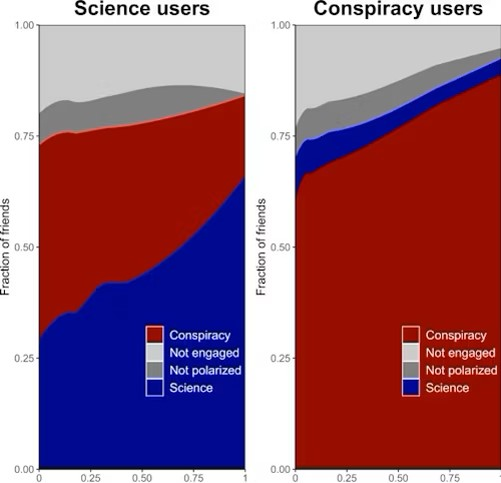
\includegraphics[width=\linewidth]{images/echo_chamber_graph_a.jpg}
		\caption{Gráfico demonstra câmara de eco entre usuários que seguem páginas de Ciência vs. Conspiraçao no Facebook e como nichos se afunilam promovendo isolamento entre usuários.}
		\fdireta{2019_Brugnoli}
		\label{fig:echo_chamber_graph_a}
	\end{subfigure}
	\hfill
	\begin{subfigure}{0.3\textwidth}
		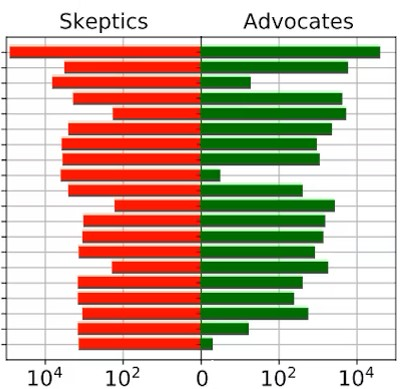
\includegraphics[width=\linewidth]{images/echo_chamber_graph_b.jpg}
		\caption{Gráfico demonstra a câmara de eco entre Céticos vs. Defensores da vacinação na Itália e como a polarização pode contribuir para a desinformação.}
		\fdireta{2020_Cossard}
		\label{fig:echo_chamber_graph_b}
	\end{subfigure}
	\hfill
	\begin{subfigure}{0.3\textwidth}
		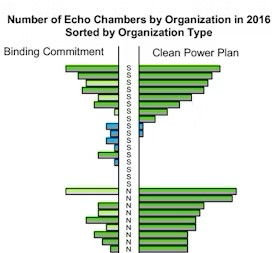
\includegraphics[width=\linewidth]{images/echo_chamber_graph_c.jpg}
		\caption{Grafico demonstra câmara de eco entre organicações no debate de políticas públicas de meio ambiente e mudanças climáticas dos EUA em 2016, especificamente sobre investir ou não em um plano de energia limpa.}
		\fdireta{2018_Jasny}
		\label{fig:echo_chamber_graph_c}
	\end{subfigure}
	\caption{Gráficos de polarização em estudos de análise de câmaras de eco.}
	\label{fig:echo_chamber_graph}
\end{figure}

Essa formação de grupos ideológicos não é meramente um reflexo da natureza humana, mas é intensificada pela arquitetura e algoritmos das plataformas digitais. Na busca por otimizar a experiência do usuário, essas plataformas frequentemente reforçam crenças preexistentes, gerando 'bolhas de filtro', conforme observado por \citeonline{2016_Flaxman}. Essas bolhas, embora possam servir como escudos contra informações perturbadoras, também restringem a exposição a uma gama diversificada de perspectivas. No entanto, a era digital não se resume apenas a câmaras de eco. \citeonline{2019_Brugnoli} destaca que em ambientes online, mecanismos cognitivos, como a evitação de desafio, viés de confirmação, dissonância cognitiva e a busca por validação, são intensificados, com a validação frequentemente a um clique de distância. Essa noção, reforça papel das mídias sociais na formação e reforço dessas fenômenos no ciberespaço.

\begin{citacao}
	'Eu defino o ciberespaço como o espaço de comunicação aberto pela interconexão mundial dos computadores e das memórias dos computadores. Essa definição inclui o conjunto dos sistemas de comunicação eletrônicos (aí incluídos os conjuntos de redes hertzianas e telefônicas clássicas), na medida em que transmitem informações provenientes de fontes digitais ou destinadas à digitalização. Insisto na codificação digital, pois ela condiciona o caráter plástico, fluido, calculável com precisão e tratável em tempo real, hipertextual, interativo e, resumindo, virtual da informação que é, parece-me, a marca distintiva do ciberespaço' \cite[p. 102]{2010_Levy_BOOK}.
\end{citacao}

\citeonline{{2010_Levy_BOOK}}, por sua vez, argumenta que as dinâmicas 'entrelaçadas' do ciberespaço refletem uma confluência de atores, projetos e interpretações, muitas vezes em oposição. O autor salienta que, apesar das tendências dominantes da era digital, a manifestação dessas tendências na vida cotidiana se dá por vários aspectos. A diversidade de interesses e perspectivas é emblemática da natureza fluida do ciberespaço. Enquanto alguns enxergam o ciberespaço como um domínio de comunicação livre e comunitária, outros o veem como um mercado global expansivo. Essas visões frequentemente colidem, ilustrando a complexidade e diversidade de vozes no ciberespaço. O autor também enfatiza que a representatividade cultural no ciberespaço é proporcional ao engajamento ativo e à qualidade das contribuições de seus participantes. 

Embora existam obstáculos à expressão da diversidade cultural, eles são menos proeminentes no ciberespaço do que em outros meios. Isso sugere que o ciberespaço, ao conectar indivíduos de diferentes origens, amplifica a diversidade de perspectivas. Em resumo, \citeonline{{2010_Levy_BOOK}} oferece uma perspectiva equilibrada e otimista sobre polarização e diversidade no ciberespaço. Ele reconhece os desafios da coexistência de múltiplas perspectivas, mas também vê o ciberespaço como um meio de expressão da diversidade cultural e colaboração. Isso sugere que, embora a polarização seja uma realidade, o ciberespaço também oferece oportunidades para diálogo e colaboração.

No contexto das plataformas digitais, a perspectiva de Lévy sobre a cibercultura é essencial para entender a dinâmica da polarização. Enquanto plataformas como o Colab podem enfrentar desafios de 'bolhas de filtro' que limitam a diversidade de perspectivas, a natureza interconectada da cibercultura, conforme descrito por Lévy, também apresenta oportunidades. Essa interconexão pode facilitar diálogos construtivos e a negociação de diferentes pontos de vista. Portanto, ao reconhecer e valorizar essa diversidade, o Colab tem o potencial de se tornar um espaço inclusivo para o diálogo cidadão.

A abordagem de Lévy sobre a cibercultura ressalta a natureza interconectada e a valorização da diversidade de perspectivas em discursos online evocam a utilização de heurísticas analíticas inovadoras que possam extrair informações estratégicas a partir dos dados de redes sociais. O Colab, além de ser um aplicativo e uma rede social de cidadania, pode ser classificado como um 'barômetro social hiperlocal'. Isso significa que, ao analisar postagens do ponto de vista de sentimentos e personas, é possível inferir a pressão social sobre determinados assuntos, relacionados a tipos específicos de eventos, de comunidades específicas em locais específicos. Assim, o 'barômetro social hiperlocal' não é uma ferramenta separada, mas sim uma caracterização do próprio Colab e de sua capacidade de mediar e refletir as nuances das opiniões e sentimentos da comunidade.

Na análise sentimento e personas das postagens do usuários do Colab, uma tendência interessante se destaca: a maioria dos usuários foi classificado como \textit{helper}, com apenas alguns nichos dominados por \textit{complainers}. Esta classificação de personas proporciona entender de forma mais matizada da comunidade, destacando áreas de colaboração positiva e pontos de tensão. O conceito de 'barômetro social hiperlocal', aliado à análise de sentimentos das postagens, adiciona uma dimensão adicional ao nosso entendimento. Ao incorporar o tipo de evento como uma variável, podemos discernir nuances na pressão social manifestada pelos usuários. Enquanto, em média, as postagens tendem a adotar um tom mais neutro, a análise focada em eventos específicos revela áreas de intensa polarização, permitindo-nos identificar e abordar tópicos de particular tensão dentro da comunidade. Com as abordagens e ferramentas certas, como aquelas inspiradas por Lévy e implementadas no Colab, há um potencial significativo para promover a participação cidadã, o engajamento e a construção de comunidades mais informadas e coesas.

\section{Dinâmicas de Pressão Social}

A análise das interações no Colab revela uma rica dinâmica de participação cidadã em eventos de zeladoria pública. Com um total de 132.858 eventos registrados, observa-se uma participação ativa de 4.569 usuários únicos, indicando uma média de aproximadamente 29 eventos por usuário. Esta média sugere um engajamento considerável dos cidadãos na plataforma, refletindo sua preocupação e envolvimento ativo em questões de zeladoria em suas comunidades.

Ao explorar a estrutura de relacionamentos entre os usuários, identificamos 25.785 conexões, ou arestas, que delineiam a rede de interações no Colab. Estas arestas representam as conexões estabelecidas entre os 6.904 nós, ou entidades, que compõem a rede. Estes nós, em sua maioria, representam os usuários e suas características demográficas e geográficas.

Em relação à distribuição geográfica, Niterói emerge como a cidade com a maior representação, contabilizando 4.246 usuários. Em seguida, temos Santo André com 1.942 usuários e Mesquita com 716. No entanto, ao analisar a distribuição de eventos por cidade, observamos uma dinâmica interessante. Mesquita, apesar de ter o menor número de usuários, lidera em termos de eventos registrados, com um total de 63.927. Niterói, com o maior número de usuários, registra 42.191 eventos, enquanto Santo André contabiliza 26.740 eventos. Esta discrepância entre o número de usuários e o número de eventos sugere variações no nível de atividade e engajamento dos usuários em diferentes cidades.

A análise dos tipos de eventos reportados nas três cidades - Mesquita, Niterói e Santo André - revela padrões distintos de preocupações e demandas dos cidadãos em cada localidade, refletindo as particularidades e desafios urbanos enfrentados por cada comunidade.

\begin{figure}[htb]
	\centering
	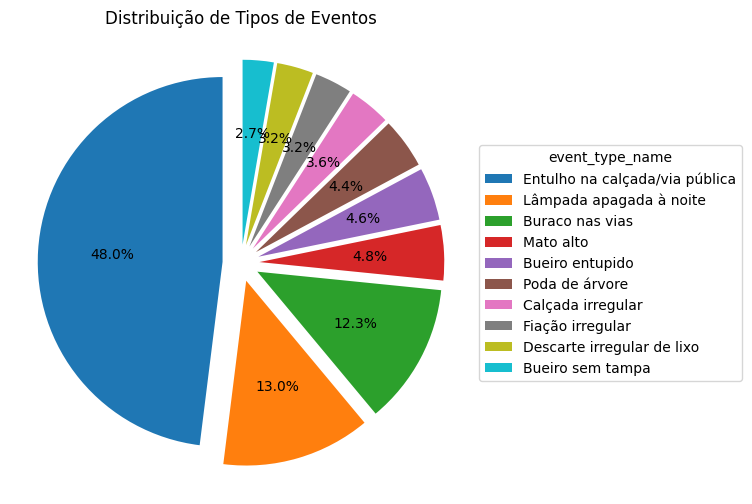
\includegraphics[width=0.7\textwidth]{images/pie_event_distribution.png}
	\caption{Distribuição dos tipos de evento mais comuns em Mesquita, Niterói e Santo André.}
	\label{fig:pie_event_distribution}
\end{figure}

Em Mesquita, o evento mais reportado, com uma expressiva quantidade de 45.235 registros, é 'Entulho na calçada/via pública'. Este número elevado sugere que a gestão de resíduos e a limpeza urbana são desafios significativos para a cidade. A presença massiva de entulho nas vias pode indicar problemas na coleta regular de lixo ou na conscientização da população sobre o descarte adequado. Além disso, eventos como 'Bueiro entupido' e 'Esgoto a céu aberto' também figuram no top 10. reforçando a ideia de que a infraestrutura urbana e os serviços de saneamento são áreas de preocupação para os cidadãos de Mesquita.

Por outro lado, em Niterói, a principal preocupação está relacionada à iluminação pública, com 'Lâmpada apagada à noite' liderando a lista. Este tipo de evento, além de estar relacionado à segurança pública, também pode afetar a qualidade de vida dos cidadãos, uma vez que áreas mal iluminadas podem desencorajar atividades noturnas e a circulação de pessoas. Adicionalmente, 'Buraco nas vias' e 'Fiação irregular' também são frequentemente reportados, indicando possíveis desafios na manutenção das vias públicas e na infraestrutura elétrica da cidade.

Em Santo André, 'Buraco nas vias' lidera as preocupações, seguido por eventos relacionados à gestão de resíduos e manutenção de áreas verdes, como 'Entulho na calçada/via pública' e 'Poda de árvore'. Estes dados sugerem que, embora haja preocupações com a infraestrutura viária, também existe uma demanda significativa por espaços urbanos mais verdes e bem cuidados.

\begin{figure}[htb]
	\centering
	\caption{10 Principais Tipos de Eventos mais criados por Cidade}\label{fig:city-events}
	\begin{subfigure}[b]{0.317\textwidth}
		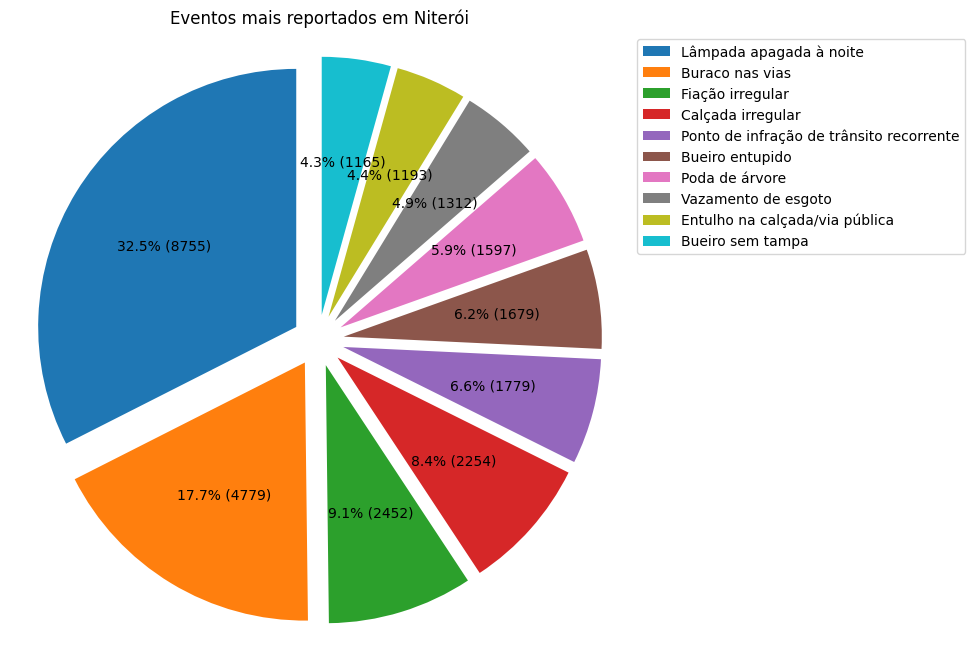
\includegraphics[width=\textwidth]{images/pie_event_distribution_niteroi.png}
		\caption{Niterói}
		\label{fig:niteroi-pie}
		\subcaption*{Em Niterói, o alto número de relatos sobre problemas como \textit{Lâmpada apagada à noite} e \textit{Buraco nas vias} pode indicar uma preocupação com a segurança noturna e a qualidade das estradas. A alta frequência desses eventos sugere a necessidade de intervenções específicas.}
	\end{subfigure} ~
	\begin{subfigure}[b]{0.317\textwidth}
		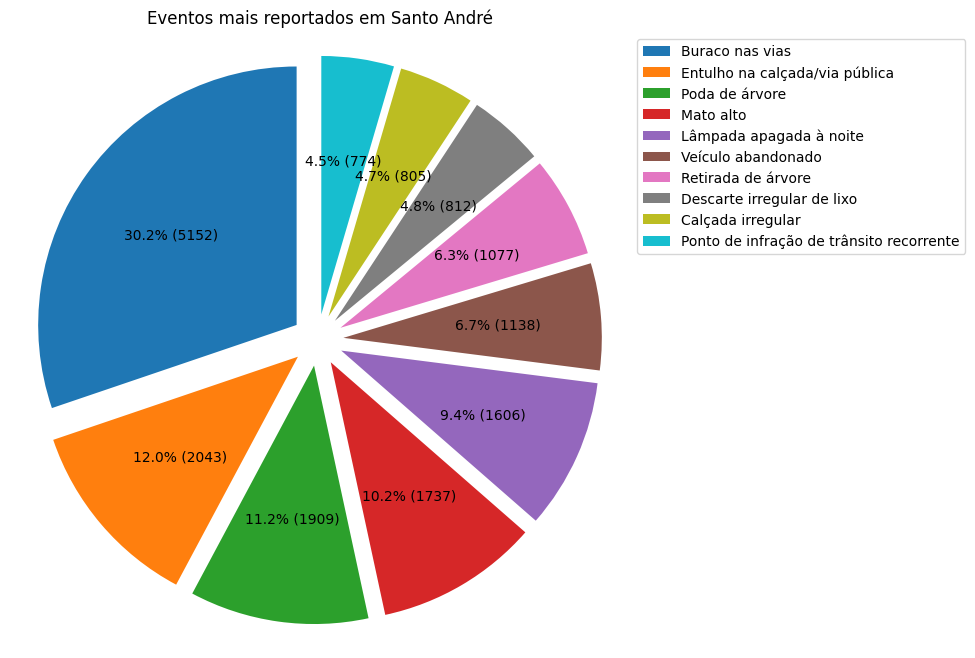
\includegraphics[width=\textwidth]{images/pie_event_distribution_sa.png}
		\caption{Santo André}
		\label{fig:santo-andre-pie}
		\subcaption*{Santo André destaca-se pela quantidade significativa de relatos sobre \textit{Buraco nas vias} e \textit{Entulho na calçada/via pública}. Esses problemas podem impactar a mobilidade urbana e a limpeza das áreas públicas. Talvez medidas de manutenção e limpeza sejam necessárias.}
	\end{subfigure} ~
	\begin{subfigure}[b]{0.317\textwidth}
		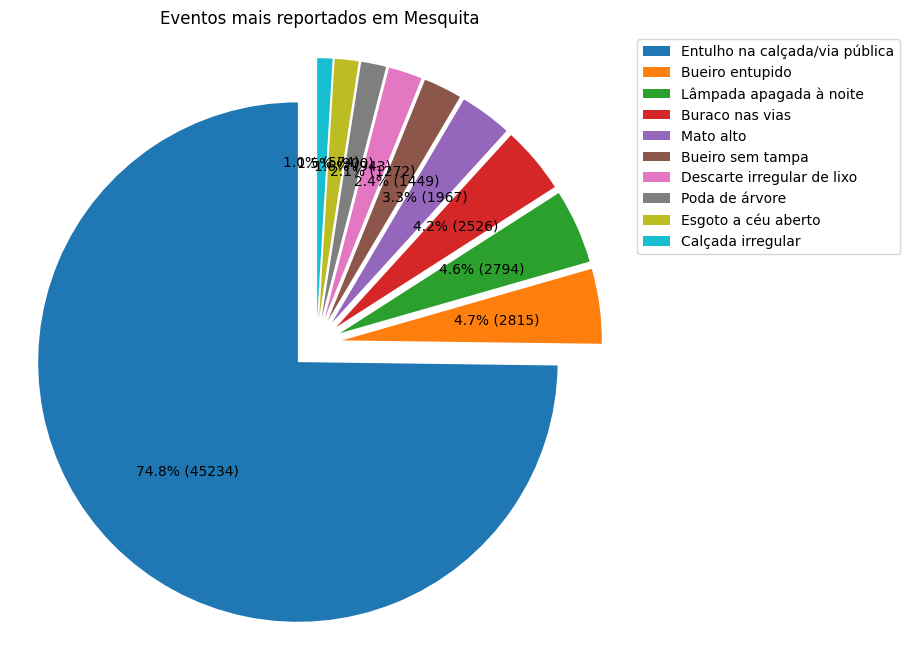
\includegraphics[width=\textwidth]{images/pie_event_distribution_mesquita.png}
		\caption{Mesquita}
		\label{fig:mesquita-pie}
		\subcaption*{Mesquita é caracterizada por um grande número de relatos sobre \textit{Entulho na calçada/via pública}, sugerindo uma preocupação com a limpeza em espaços públicos. A alta incidência desse problema pode indicar a necessidade de iniciativas de limpeza e conscientização.}
	\end{subfigure}
\end{figure}


Estas variações nas principais preocupações reportadas em cada cidade refletem a diversidade de desafios urbanos enfrentados por diferentes comunidades. A pressão social, como medida pela frequência e tipo de eventos reportados, serve como um indicativo das áreas que requerem atenção prioritária das autoridades locais. Ao mesmo tempo, a capacidade dos cidadãos de reportar e categorizar eventos em plataformas como o Colab permite uma compreensão mais aprofundada das dinâmicas locais, oferecendo uma ferramenta valiosa para a tomada de decisões informadas.

Além disso, a análise desses eventos também pode fornecer insights sobre a eficácia das políticas públicas em vigor. Por exemplo, um aumento súbito no número de eventos relacionados a 'Buraco nas vias' após uma temporada de chuvas pode indicar a necessidade de melhorias na infraestrutura viária. Da mesma forma, um número elevado de reportagens sobre 'Entulho na calçada/via pública' pode sinalizar a necessidade de campanhas de conscientização sobre descarte adequado ou de melhorias nos serviços de coleta de resíduos.

\section{Heurísticas para cálculo da Pressão Social Hiperlocal}

Nesta seção, abordaremos as heurísticas desenvolvidas para quantificar a pressão ou polaridade dos discursos nas postagens de eventos de zeladoria pública no Colab. Estas heurísticas, originadas de uma combinação de literatura existente e insights práticos, se tornaram cruciais para entender a opinião média de um grupo de usuários sobre eventos específicos de zeladoria pública. Elas são essenciais para medir a pressão social em comunidades hiperlocais, fornecendo insights valiosos para tomadores de decisão, pesquisadores e outros stakeholders interessados em compreender as complexas dinâmicas urbanas.

A relevância dessas heurísticas reside na sua capacidade de capturar a essência das opiniões dos cidadãos em contextos urbanos específicos. Ao analisar os tipos de eventos e as dinâmicas de participação cidadã na plataforma, podemos identificar tendências, preocupações e áreas de interesse, auxiliando na tomada de decisões informadas.

O conjunto de dados utilizado para esta análise foi meticulosamente compilado. Identificamos todos os usuários que fazem parte das comunidades da rede, conforme detalhado no \autoref{chapter:05_exploratory}, das cidades de Niterói, Santo André e Mesquita na rede Colab. Posteriormente, todas as postagens disponíveis desses usuários em eventos de zeladoria pública foram analisadas. Utilizamos o modelo de classificação descrito no \autoref{chapter:06_sentiment} para prever a persona do usuário e atribuir um score de sentimento a cada postagem. Esta metodologia nos permitiu obter insights sobre o comportamento dos usuários, como a expressão de suas opiniões e sentimentos. Adicionalmente, categorizamos os tipos de eventos associados a cada postagem.

\begin{table}[htbp]
	\centering
	\caption{Modelo de Dados para Análise de Pressão Social Hiperlocal}
	\begin{tabular}{ll}
		\toprule
		\textbf{Campo}    & \textbf{Descrição}                                  \\
		\midrule
		event\_id         & Identificador único do evento                       \\
		colab\_user\_id   & Identificador único do usuário do Colab             \\
		score             & Score de sentimento atribuído à postagem do usuário \\
		persona\_value    & Persona prevista para o usuário que fez a postagem  \\
		event\_type\_id   & Identificador único do tipo de evento               \\
		event\_type\_name & Nome descritivo do tipo de evento                   \\
		\bottomrule
	\end{tabular}
	\label{tab:modelo-dados-barometro}
\end{table}

Na \autoref{tab:modelo-dados-barometro}, cada linha representa uma postagem no Colab e inclui informações como o ID do evento, o ID do usuário do Colab, a pontuação de sentimento associada à postagem, a persona atribuída ao usuário que a fez, o ID do tipo de evento e o nome do tipo de evento relacionado. Esses dados formam a base essencial para nossas análises, permitindo-nos calcular a pressão social hiperlocal e compreender as dinâmicas das preocupações urbanas nessas comunidades específicas.

Com base neste modelo de dados, iniciamos o processo de filtragem e agregação. Primeiro, focamos nos membros ativos das comunidades identificadas na análise exploratória conduzida no \autoref{chapter:05_exploratory}. Em seguida, selecionamos tipos de eventos específicos, agrupados por tema, para nossa análise. Esta seleção foi guiada pela intenção de avaliar a pressão social hiperlocal em relação a preocupações específicas de zeladoria pública. Após a filtragem, calculamos duas métricas-chave para cada tipo de evento: a pontuação média de sentimento e a persona média. A primeira reflete o sentimento médio das postagens, enquanto a segunda representa a distribuição média das personas dos usuários. Essas métricas são calculadas para cada tipo de evento, permitindo-nos comparar e analisar as diferenças entre eles.

A visualização da pressão social hiperlocal é apresentada através de um gráfico de radar, uma representação gráfica que permite analisar e comparar diversas variáveis em relação a um ponto central. O gráfico possui dois planos distintos: o plano de score e o plano de persona.

\begin{quadro}[htb]
	\centering
	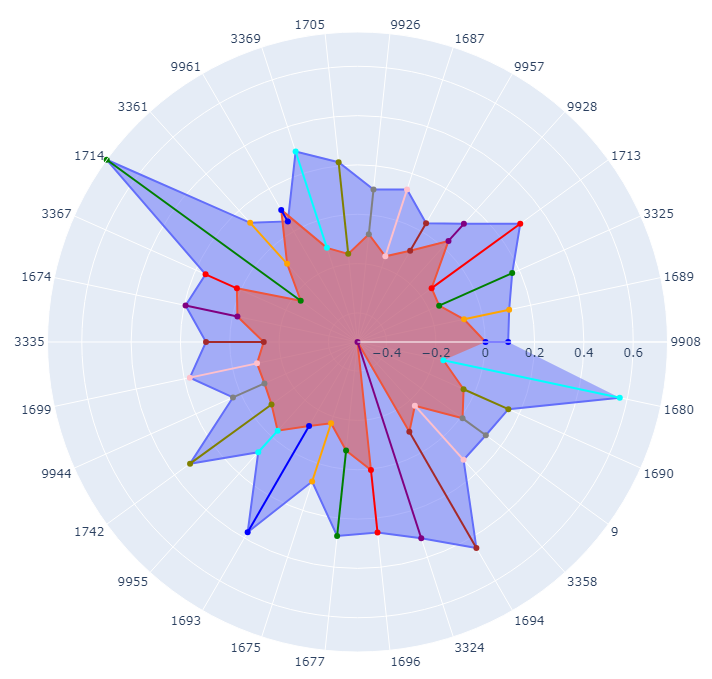
\includegraphics[width=0.7\textwidth]{images/social_barometer_plot.png}
	\caption{Gráfico de Radar para Análise de Pressão Social Hiperlocal. Os segmentos representam tipos de eventos, enquanto o eixo radial exibe valores médios de scores de sentimentos (plano vermelho) e personas (plano azul) atribuídos às postagens dos usuários relacionadas a cada tipo de evento.}
	\label{fig:social_barometer_plot}
\end{quadro}

No plano de score, cada segmento do gráfico de radar representa um tipo específico de evento do Colab, onde cada evento é associado a um ângulo theta. O eixo radial, representado pelo parâmetro 'R', indica o valor médio dos scores de sentimentos atribuídos às postagens dos usuários em relação a um determinado tipo de evento. Quanto mais distante do centro estiver um segmento, maior será o valor médio do score e, consequentemente, mais positivo será o sentimento expresso pelos usuários em relação a esse evento. Por outro lado, segmentos mais próximos do centro indicam scores médios mais baixos, refletindo sentimentos mais negativos.

No plano de persona, novamente, cada segmento do gráfico representa um tipo de evento, O eixo radial 'R' neste caso indica o valor médio das personas previstas dos usuários em relação ao tipo de evento. Quanto mais próximo de 0 estiver um segmento, mais os usuários tendem a assumir uma persona de \textit{helper}, caracterizada por atitudes positivas e colaborativas em relação ao evento. À medida que o valor de 'R' se aproxima de 1, os usuários tendem a adotar uma persona de \textit{complainer}, indicando uma postura mais crítica e insatisfeita. Essa representação gráfica única proporciona uma visão abrangente e comparativa das opiniões e personas dos usuários do Colab em relação a diferentes tipos de eventos, permitindo uma análise mais profunda das dinâmicas das comunidades hiperlocais.

Após a definição do modelo de dados e a coleta das postagens no Colab, começamos a formulação das heurísticas que conduziriam à análise da pressão social hiperlocal. Esta etapa foi crucial, pois a vastidão e variedade dos dados requeriam um direcionamento para captar efetivamente as nuances das dinâmicas urbanas. O primeiro passo foi a identificação dos tópicos de interesse. Escolhemos tópicos que são comumente discutidos em comunidades urbanas e têm um impacto direto na qualidade de vida dos cidadãos. Um exemplo elucidativo dessa seleção é o tópico 'Tarifa de Transporte Público'. 

A escolha desse tema não se deu apenas pela sua manifesta relevância em discussões urbanas e pelo impacto direto que exerce no cotidiano financeiro e rotineiro dos cidadãos, mas também por sua ressonância histórica. Na história recente do Brasil, podemos remeter a um período de turbulência política, cujo estopim foi justamente o descontentamento popular em relação ao aumento das tarifas de transporte. Em junho de 2013, uma série de protestos, inicialmente convocados contra o aumento das passagens, ganhou magnitude e se espalhou por diversas cidades do país. Rapidamente, as manifestações incorporaram uma variedade de pautas e descontentamentos, culminando em uma das maiores mobilizações populares das últimas décadas no Brasil. Esse evento histórico ilustra a capacidade do tema 'Tarifa de Transporte Público' de catalisar discussões mais amplas e mobilizar grandes contingentes da população em torno de demandas comuns.

Para cada tópico escolhido, definimos um conjunto de palavras-chave. Estas palavras-chave são termos ou expressões frequentemente associados ao tópico em questão. No caso do tópico 'Tarifa de Transporte Público', palavras como 'lotado', 'ônibus', 'metrô', 'tarifa' e 'aumento da tarifa' foram consideradas. Essas palavras-chave funcionam como um filtro inicial, permitindo-nos identificar postagens no Colab que possam estar relacionadas ao tópico em análise. Com as palavras-chave definidas, realizamos uma busca nas postagens para identificar os tipos de eventos associados a elas. Esta busca retorna uma variedade de eventos, que podem ou não estar diretamente relacionados ao tópico de interesse.

Por exemplo, uma postagem que menciona 'passagem está cara' em um contexto de 'ônibus danificado' sugere uma intersecção do tópico de 'Tarifa de Transporte Público' com um evento relacionado. Isso indica que o usuário está manifestando sua insatisfação com o serviço, relacionando o valor pago à qualidade recebida. Para refinar ainda mais nossa análise, criamos uma lista de eventos não relevantes, que são excluídos da análise final. Esta lista foi elaborada com base em nossa compreensão do tópico e na intuição de quais eventos poderiam desviar o foco da pressão social que queríamos captar. No exemplo anterior, os eventos como 'Ponto de infração de trânsito recorrente' e 'Rampa de acessibilidade irregular ou inexistente' foram considerados na análise, pois, mesmo não sendo diretamente sobre tarifas, são eventos que afetam a experiência do usuário no transporte público.

Após a filtragem e seleção, calculamos métricas para os eventos restantes, como pontuação média de sentimento e persona média. A combinação dessas métricas, associadas aos eventos filtrados, nos fornece um panorama da pressão social em relação ao tópico analisado. Essa abordagem, que combina a seleção de tópicos, identificação por palavras-chave e filtragem de eventos, permite-nos isolar e analisar os sentimentos e opiniões dos usuários em relação a questões urbanas específicas, proporcionando insights valiosos sobre as dinâmicas das comunidades urbanas.

\section{Tópicos de Pressão Social}

O Colab é uma plataforma de participação cidadã que proporciona um espaço virtual para os cidadãos expressarem suas preocupações, compartilharem experiências e debaterem questões urbanas relevantes. Neste ambiente, emergem tópicos de pressão social que refletem as preocupações específicas dos cidadãos. A escolha desses tópicos foi baseada não apenas na sua frequência de aparição na plataforma, mas também na sua relevância para as políticas públicas urbanas e na amplitude de impacto que podem ter nas comunidades. Ao escolher esses tópicos, procuramos abordar tanto questões mais generalizadas, como saúde e segurança, quanto questões emergentes e altamente debatidas, como gentrificação e higienismo social. Esses tópicos desempenham um papel fundamental na compreensão dos desafios enfrentados nas cidades.

Em uma plataforma como o Colab, as preocupações dos cidadãos podem ser expressas de maneira apaixonada e, por vezes, polarizada. Através de uma busca por palavras-chave específicas, identificamos e categorizamos diversos desses tópicos de pressão social que surgem nas discussões e associamos eventos de zeladoria pública a esses tópicos. Agora, nosso objetivo é analisar esses tópicos sob a perspectiva do Colab como um 'Barômetro Social Hiperlocal', investigando como eles impactam a dinâmica da plataforma e fornecem informações valiosas para decisores, pesquisadores e comunidades e munícipes. As métricas de pressão social organizadas por tipo de evento e contendo número de eventos criados, score médio de sentimento e persona média identificada estão disponíveis no \autoref{chapter:tables_social_pressure}.

\subsection{Mobilidade Urbana}
\label{section:mobilidade-urbana}

\begin{figure}[htb]
	\centering
	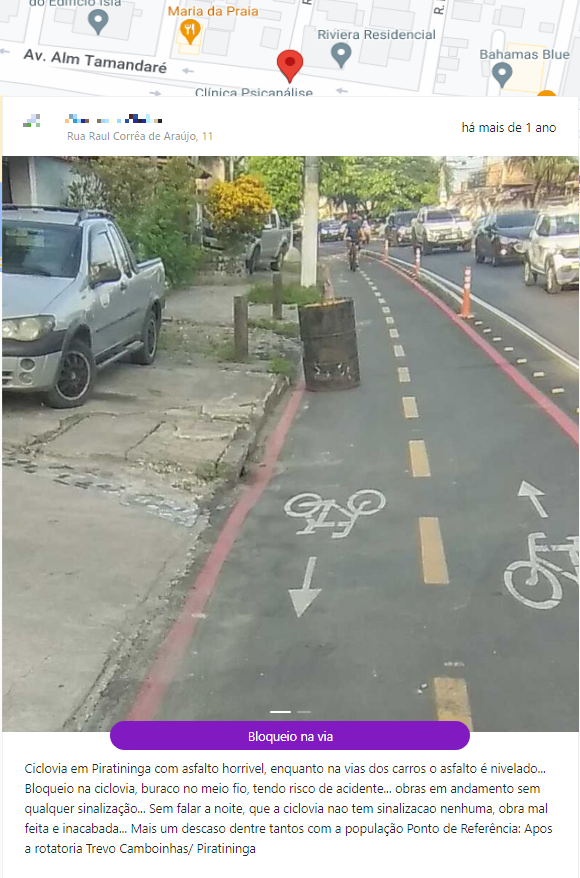
\includegraphics[width=0.7\textwidth]{images/colab_posts_mobility.png}
	\caption{Usuário do Colab expressando insatisfação com a qualidade da ciclofaixa em comparação com a rua de automóveis.}
	\label{fig:colab_posts_mobility}
\end{figure}

A mobilidade urbana é um tópico essencial nas cidades modernas, especialmente com o crescimento das populações urbanas e os desafios enfrentados pelos sistemas de transporte. Na plataforma colaborativa Colab, cidadãos discutem intensamente sobre este tema, refletindo a era das 'smart cities' e 'connected citizens'. As opiniões se polarizam entre preferências por transporte pessoal, transporte público, ciclovias e caminhadas. Questões ambientais, como a redução das emissões de carbono, e temas de acessibilidade e equidade também dividem opiniões, influenciando debates sobre planejamento urbano e alocação de recursos.

As métricas de pressão sociais disponíveis na \autoref{tab:eventos_populares_mobility} destacam uma série de eventos relacionados à mobilidade urbana, cada um com um número significativo de ocorrências e variações notáveis nos scores de sentimento e personas. Entre os eventos mais frequentes, 'Bloqueio na via' e 'Ponto de infração de trânsito recorrente' aparecem 16 vezes cada, ambos com scores negativos de -0.2272 e -0.2458, respectivamente, indicando uma percepção predominantemente negativa dos usuários. A persona associada a esses eventos é alta, sugerindo que esses eventos são frequentemente reportados por indivíduos que se sentem fortemente inclinados a expressar sua insatisfação.

Por outro lado, 'Entulho na calçada/via pública' possui um score relativamente menos negativo de -0.0303, refletindo uma reação menos intensa dos usuários. Eventos como 'Bueiro sem tampa' e 'Manutenção de ciclovia/ciclofaixa' apresentam os scores de sentimento mais negativos, -0.3101 e -0.2643, respectivamente, indicando preocupações significativas com a infraestrutura urbana. A análise das personas mostra que eventos como 'Ponto de transporte clandestino' têm uma persona muito alta (0.9333), indicando uma forte tendência dos usuários de reportar esses problemas específicos. No geral as métricas de pressão social revelam uma preocupação comum com a manutenção e segurança das vias públicas, refletindo uma pressão social significativa sobre esses tópicos.

\begin{figure}[htb]
	\centering
	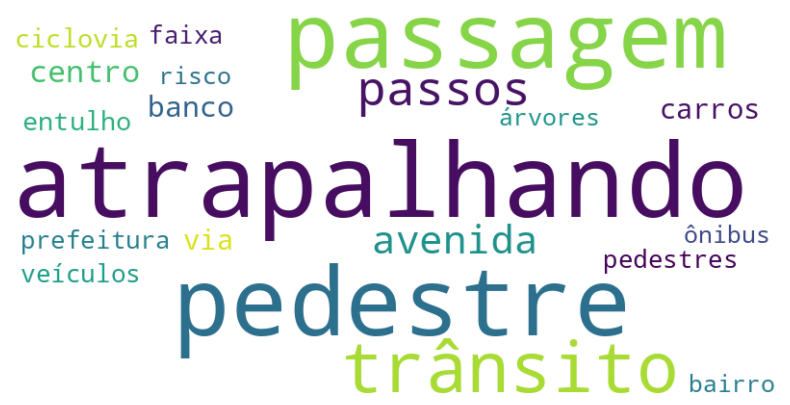
\includegraphics[width=0.7\textwidth]{images/wordcloud_mobility.png}
	\caption{Wordcloud com palavras mais frequentes em postagens sobre mobilidade urbana}
	\label{fig:wordcloud_mobility}
\end{figure}

\begin{quadro}[htb]
	\centering
	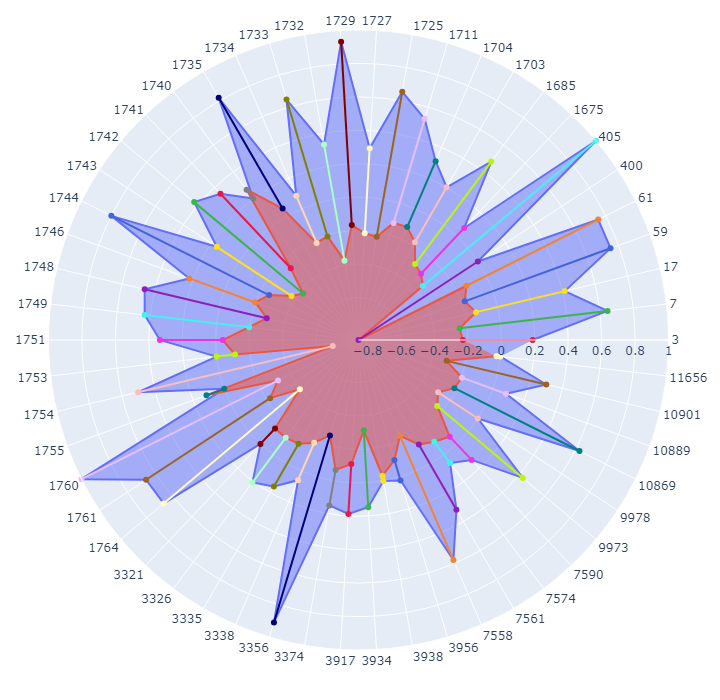
\includegraphics[width=0.7\textwidth]{images/social_barometer_mobility.png}
	\caption{Gráfico de Radar ilustrando a pressão social em relação à mobilidade urbana. O eixo radial mostra os scores de sentimentos (plano vermelho) e personas (plano azul), enquanto os segmentos descrevem diversos eventos urbanos.}
	\label{fig:social_barometer_mobility}
\end{quadro}

\subsection{Infrações de Trânsito}
\label{sec:eventos_populares_traffic}

\begin{figure}[htb]
	\centering
	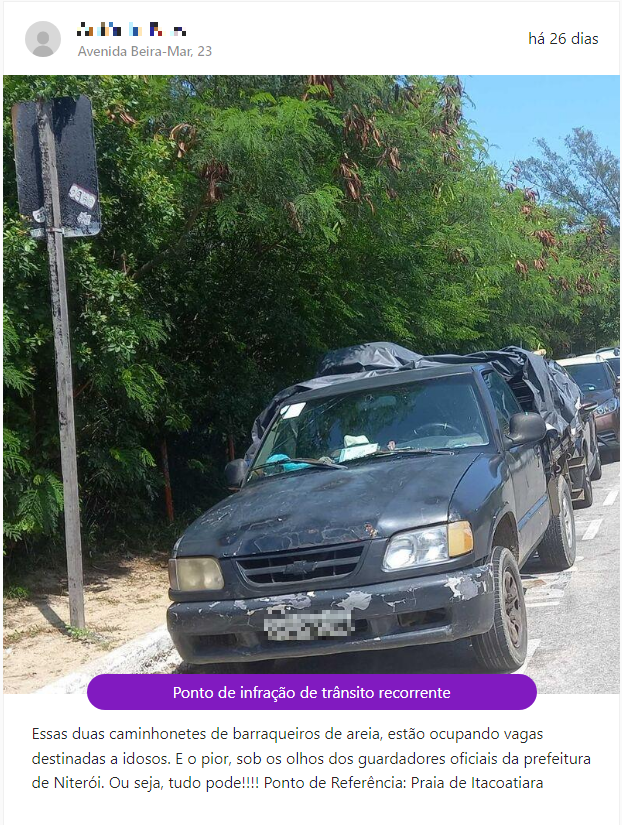
\includegraphics[width=0.7\textwidth]{images/colab_posts_traffic.png}
	\caption{Usuário do Colab expressando sua opinião sobre infrações de trânsito.}
	\label{fig:colab_posts_traffic}
\end{figure}

No tópico de infrações de trânsito, a análise de dados mostra um padrão complexo na percepção dos cidadãos sobre as ações das autoridades de trânsito. As métricas disponíveis na \autoref{tab:eventos_populares_traffic} demonstram uma clara dicotomia: por um lado, muitos acham que as autoridades poderiam fazer mais para resolver as infrações; por outro, alguns veem as autoridades como excessivamente punitivas, criando uma 'indústria da multa'. Palavras-chave como 'multa', 'infração', 'detran' e 'IPVA' são frequentemente mencionadas, indicando preocupações com penalidades e questões burocráticas.

\begin{figure}[htb]
	\centering
	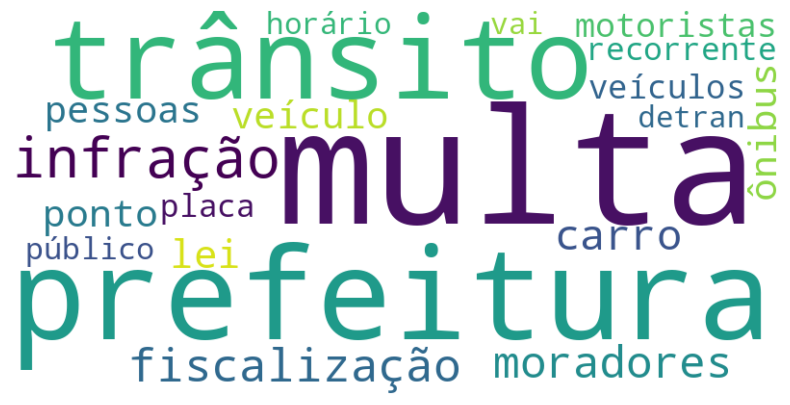
\includegraphics[width=0.7\textwidth]{images/wordcloud_traffic.png}
	\caption{Wordcloud com palavras mais frequentes em postagens sobre infrações de trânsito}
	\label{fig:wordcloud_traffic}
\end{figure}

Ao analisar sentimentos e perspectivas sobre infrações, nota-se uma diversidade de reações. Alguns tópicos como 'Conservação (via pública)' e 'Via de terra com desnível' recebem sentimentos positivos, sugerindo satisfação com medidas adotadas. Em contraste, questões como 'Manutenção de faixa de pedestre' e 'Ônibus/trem/metrô danificado' têm sentimentos negativos, indicando insatisfação. Além disso, problemas como 'Rampa de acessibilidade irregular' e 'Bueiro sem tampa' tendem a gerar críticas, enquanto questões como 'Retirada de árvore' e 'Conservação (via pública)' veem posturas mais colaborativas.

\begin{quadro}[htb]
	\centering
	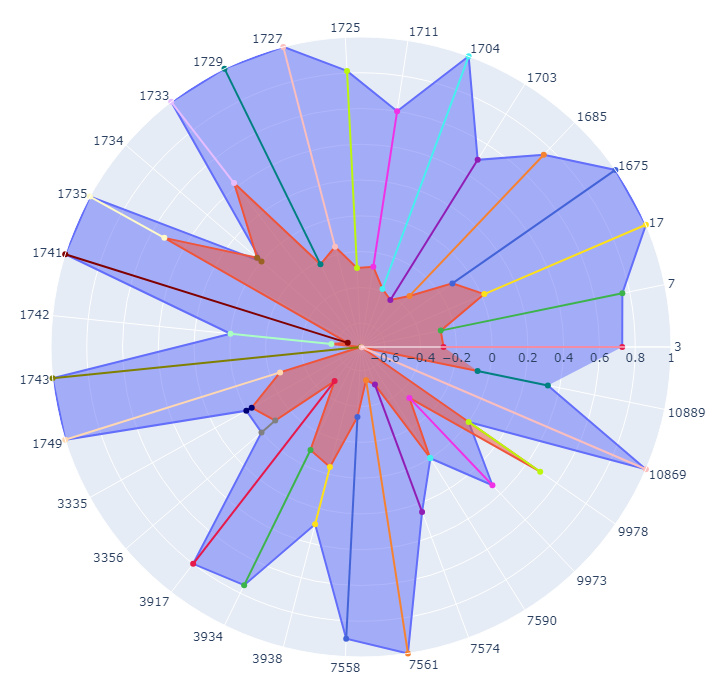
\includegraphics[width=0.7\textwidth]{images/social_barometer_traffic.png}
	\caption{Gráfico de Radar ilustrando a pressão social em relação ao tópico de Infrações de Trânsito.}
	\label{fig:social_barometer_traffic}
\end{quadro}

Esses dados mostram que as preocupações dos cidadãos com infrações de trânsito vão além das multas, abrangendo a eficiência das autoridades e a qualidade de vida urbana. O alto engajamento em tópicos como multas e zonas de infração recorrente revela um interesse significativo da comunidade nesses assuntos. A pressão social reflete uma mistura de críticas construtivas e insatisfação, destacando a diversidade de opiniões e a complexidade das dinâmicas sociais relacionadas às infrações de trânsito.

\subsection{Tarifa de Transporte Público}
\label{sec:eventos_populares_busfare}

\begin{figure}[htb]
	\centering
	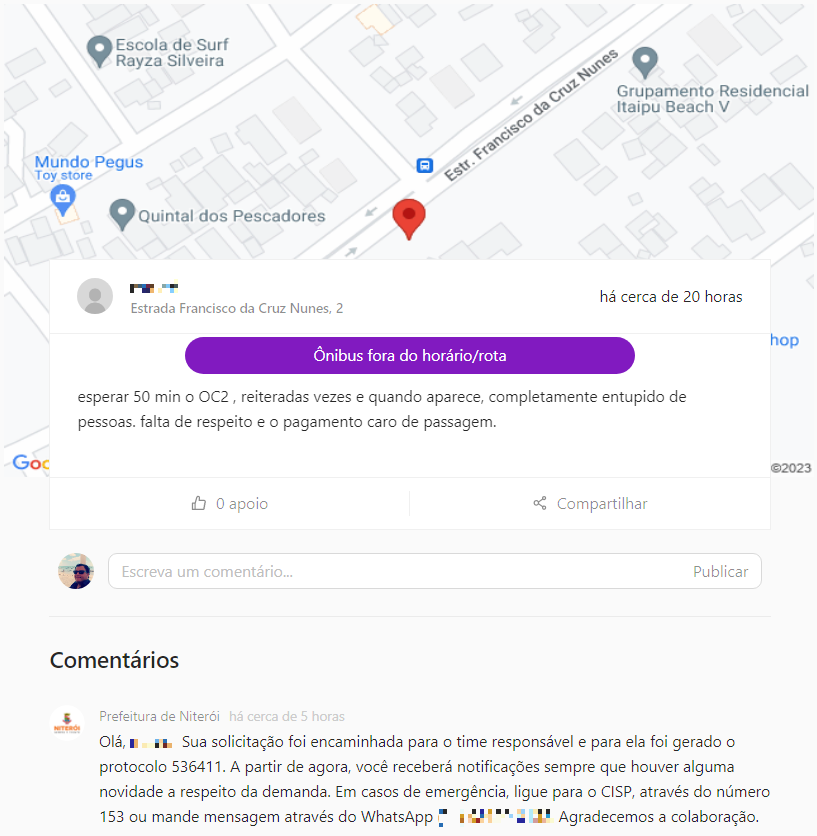
\includegraphics[width=0.7\textwidth]{images/colab_posts_busfare.png}
	\caption{Exemplo de postagem no Colab relacionadas ao tópico de Tarifa de Transporte Público}
	\label{fig:colab_posts_busfare}
\end{figure}

No contexto da tarifa de transporte público, os dados da \autoref{tab:eventos_populares_busfare} mostram que este é um tópico de grande preocupação para os cidadãos. Palavras-chave como 'passagem', 'ônibus', 'terminal' e 'cobertura' indicam foco nas questões de custo e acessibilidade do transporte público. Muitas das postagens relacionadas a este tópico expressam insatisfação, como é evidenciado pelas menções frequentes a 'Ônibus superlotado' e 'Ônibus fora do horário/rota', com sentimentos majoritariamente negativos e uma tendência dos usuários a se expressarem como críticos (perfil de \textit{complainer}).

\begin{figure}[htb]
	\centering
	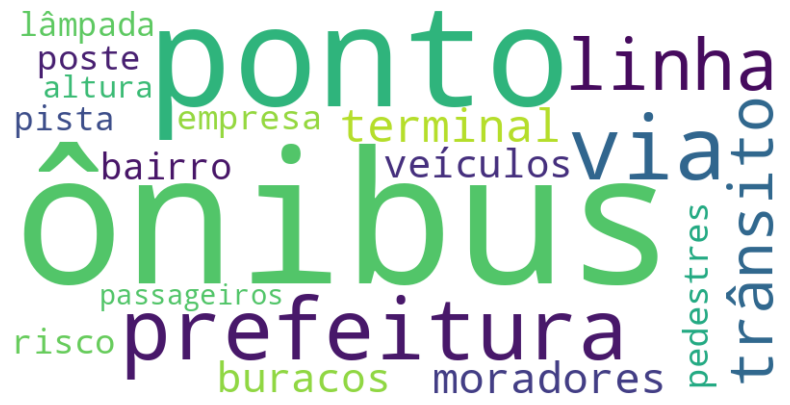
\includegraphics[width=0.6\textwidth]{images/wordcloud_busfare.png}
	\caption{Wordcloud com palavras mais frequentes em postagens sobre infrações de trânsito}
	\label{fig:wordcloud_busfare}
\end{figure}

Por outro lado, há sinais de disposição para colaborar em resolver problemas relacionados ao transporte público, especialmente em tópicos como 'Conservação (via pública)' e 'Faixa de pedestre apagada', onde os sentimentos são menos negativos e a tendência é para um perfil mais colaborativo (perfil de \textit{helper}).

\begin{quadro}[htb]
	\centering
	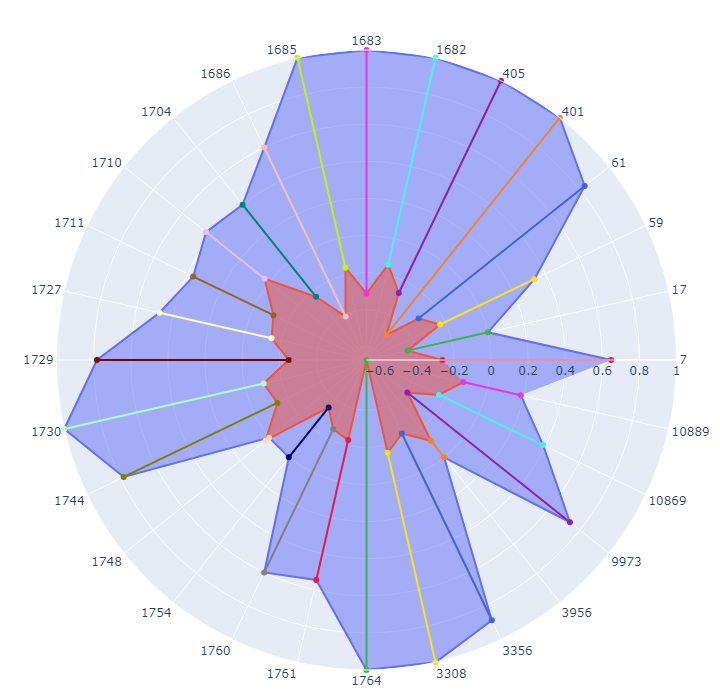
\includegraphics[width=0.7\textwidth]{images/social_barometer_bus_fare.png}
	\caption{Gráfico de Radar ilustrando a pressão social em relação ao tópico de Tarifa de Transporte Público}
	\label{fig:social_barometer_bus_fare}
\end{quadro}

A frequência do termo 'passagem' sugere uma preocupação especial com os custos do transporte, enquanto a prevalência do termo 'ônibus' em comparação com 'metrô' indica que os problemas com ônibus são mais relatados ou percebidos como mais críticos. Nos casos de eventos descritos como 'Agentes e Operadores de trânsito' ou 'Metrô/trem danificado', a postura é predominantemente crítica, com sentimentos negativos, apontando para áreas que podem necessitar de atenção imediata por parte das autoridades. Em contraste, questões como 'Manutenção de pintura da via' e 'Banco danificado' geram reações mais colaborativas, mesmo que menos frequentes, indicando que em certas situações, os cidadãos estão dispostos a oferecer feedback construtivo.

Em resumo, a discussão sobre tarifas de transporte público não se limita a ser um tópico de debate intenso; ela também abre caminho para uma colaboração significativa entre os cidadãos e as autoridades. Isso implica um potencial valioso para uma parceria construtiva na busca de melhorias no serviço de transporte público.

Para a administração das cidades, isso significa que há uma oportunidade de aproveitar esse engajamento cívico para melhorar os serviços de transporte. Os dados coletados das discussões dos cidadãos fornecem insights específicos sobre os problemas enfrentados pelos usuários do transporte público, como superlotação, inconsistências de horários e condições das infraestruturas. Ao analisar esses dados, as autoridades podem identificar as áreas mais críticas que necessitam de atenção imediata.

Por exemplo, questões frequentemente mencionadas, como a superlotação dos ônibus, podem indicar a necessidade de aumentar a frequência das viagens ou adicionar mais veículos nas rotas mais movimentadas. Da mesma forma, reclamações sobre o estado de conservação dos veículos ou infraestruturas (como terminais e estações) podem guiar os esforços de manutenção e investimento.

Utilizar esses dados também pode auxiliar no planejamento de políticas de transporte mais inclusivas e sustentáveis. Por exemplo, entender as preocupações sobre tarifas pode ajudar a modelar estruturas de preços mais equitativas e considerar alternativas como subsídios para grupos vulneráveis. Portanto, essse tópico social não é somente termômetro das percepções e experiências dos cidadãos, mas também uma bússola para direcionar políticas públicas e investimentos de maneira mais informada e responsiva às necessidades da comunidade.

\subsection{Saúde Pública}
\label{sec:eventos_populares_public_health}

\begin{figure}[htb]
	\centering
	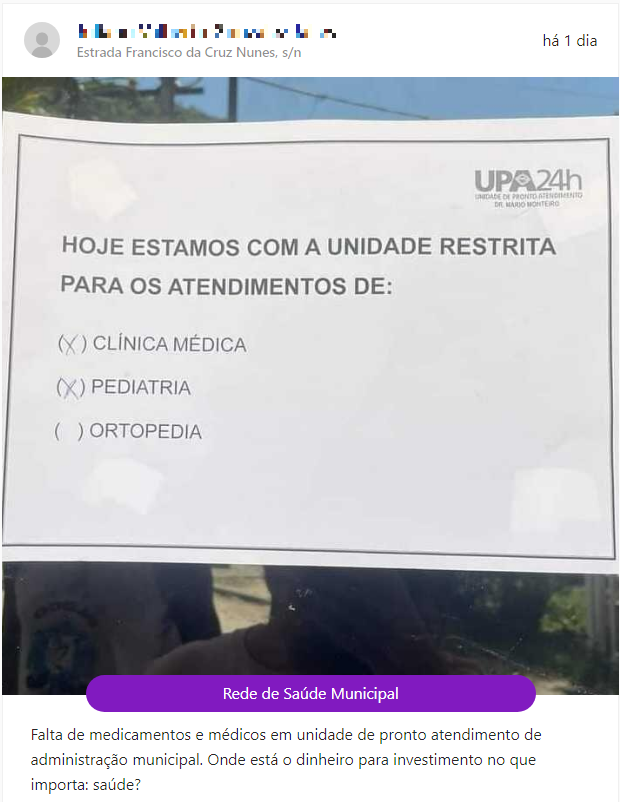
\includegraphics[width=0.7\textwidth]{images/colab_posts_health.png}
	\caption{Exemplo de postagem no Colab relacionada ao tópico de Saúde Pública}
	\label{fig:colab_posts_health}
\end{figure}

A saúde pública é um tópico crucial para as comunidades, como demonstram os dados da \autoref{tab:eventos_populares_public_health}. Palavras-chave como 'samu', 'ambulância', 'médico' e 'vacina' são frequentemente mencionadas, destacando a importância dos serviços de saúde. Termos como 'dengue' e 'zika' apontam para preocupações com doenças emergentes. Questões ambientais, como 'Foco de mosquito da dengue/zika' e 'Descarte irregular de lixo', também são proeminentes, indicando problemas de saúde relacionados ao meio ambiente.

\begin{figure}[htb]
	\centering
	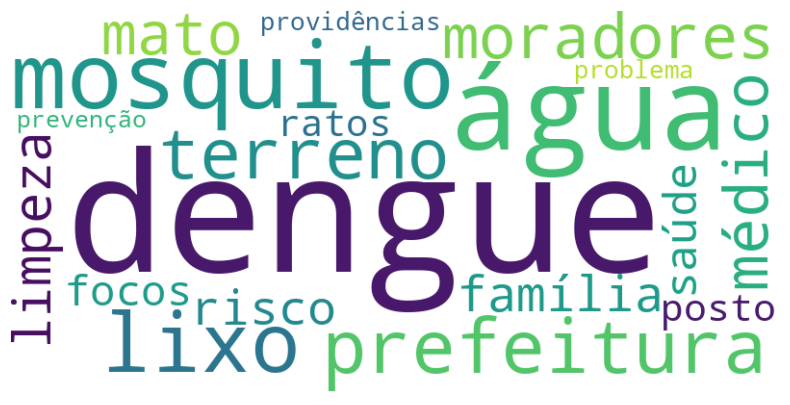
\includegraphics[width=0.7\textwidth]{images/wordcloud_public_health.png}
	\caption{Wordcloud com palavras mais frequentes em postagens sobre Saúde Pública}
	\label{fig:wordcloud_public_health}
\end{figure}

A análise mostra sentimentos majoritariamente negativos em relação a problemas como poluição sonora e descarte irregular de lixo, embora alguns eventos, como 'Atendimento na Clínica da Família', apresentem uma perspectiva mais positiva. Este contraste reflete uma diversidade de opiniões e preocupações na comunidade.

\begin{quadro}[htb]
	\centering
	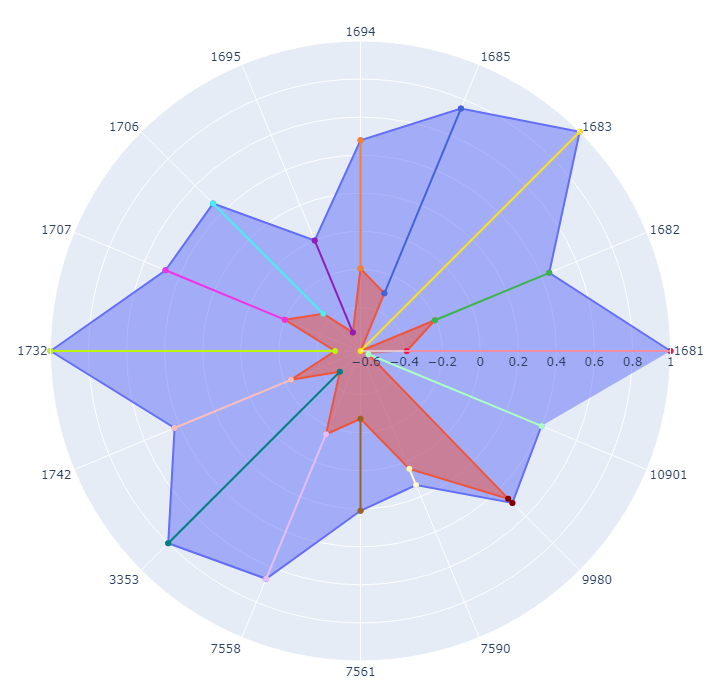
\includegraphics[width=0.7\textwidth]{images/social_barometer_public_health.png}
	\caption{Gráfico de Radar ilustrando a pressão social em relação ao tópico de Saúde Pública.}
	\label{fig:social_barometer_public_health}
\end{quadro}

Na administração urbana, a análise da saúde publica sob uma perspectiva de pressão social pode ser fundamental para aprimorar os serviços oferecidos à população. Primeiramente, o entendimento das preocupações específicas dos cidadãos, evidenciado pela análise de dados, permite que as autoridades foquem na melhoria dos serviços mais criticados. Por exemplo, a eficiência do Serviço de Atendimento Móvel de Urgência (SAMU) e a disponibilidade de vacinas são aspectos que podem ser significativamente aprimorados com base no feedback coletado. Esse foco direcionado não apenas melhora a qualidade do atendimento em saúde, mas também aumenta a confiança da população nos serviços públicos.

Além disso, a identificação frequente de doenças endêmicas, como dengue e zika, nos dados sugere a necessidade urgente de campanhas eficazes de prevenção e controle de vetores. O planejamento dessas campanhas pode ser otimizado ao se considerar as áreas e questões mais mencionadas pelos cidadãos, garantindo uma ação direcionada e mais eficiente. A conscientização e educação da população acerca dessas doenças também se torna mais focada e impactante.

A análise detalhada dos sentimentos e personas revela as atitudes variadas dos cidadãos, fornecendo informações valiosas para moldar respostas e políticas públicas alinhadas com as expectativas da comunidade. Essa abordagem baseada em dados permite uma resposta mais sensível e adaptada às necessidades específicas da população, resultando em uma administração mais eficaz e empática.

Por fim, o engajamento cívico, incentivado através de plataformas de diálogo entre cidadãos e autoridades, fortalece a participação comunitária na saúde pública. Esta abordagem colaborativa não só contribui para a resolução de problemas, mas também promove uma maior transparência e responsabilidade nas decisões públicas. Além disso, o uso de plataformas digitais para captar a voz da população se destaca como uma ferramenta crucial, permitindo uma gestão pública mais inclusiva e alinhada às necessidades reais da comunidade. Essa interação dinâmica entre cidadãos e gestores é essencial para construir cidades mais resilientes e inclusivas, onde a saúde pública é uma prioridade compartilhada e ativamente perseguida por todos os envolvidos.

\subsection{Distanciamento Social}
\label{sec:eventos_populares_social_distancing}

\begin{figure}[htb]
	\centering
	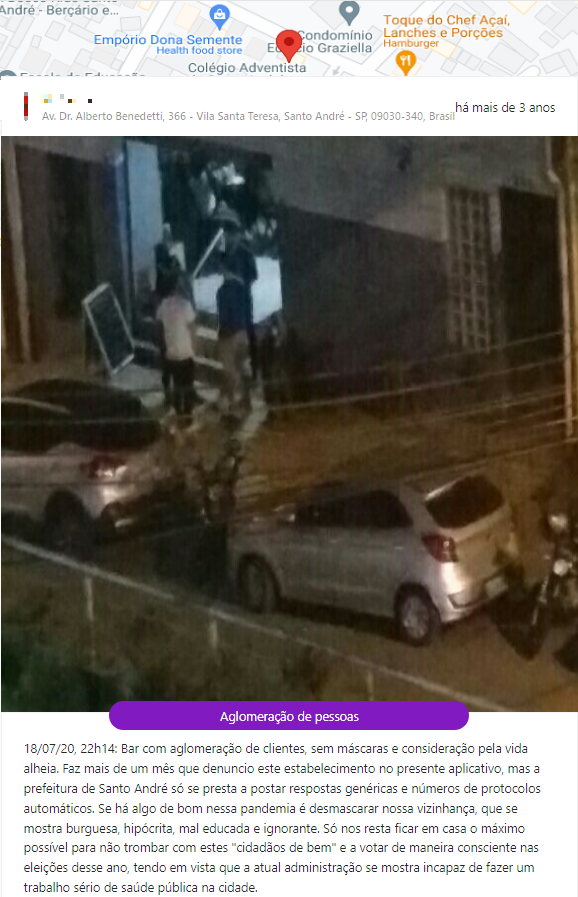
\includegraphics[width=0.7\textwidth]{images/colab_posts_social_distancing.png}
	\caption{Exemplo de postagem no Colab denunciando aglomeração de pessoas na pandemia.}
	\label{fig:colab_posts_social_distancing}
\end{figure}

A análise dos dados coletados no Colab sobre distanciamento social durante a pandemia de COVID-19 oferece insights valiosos para a administração pública. As discussões refletem a sensibilidade das comunidades à pandemia e a importância da conscientização sobre medidas de saúde, como aglomerações e uso de máscaras. Essas informações são cruciais para a implementação de estratégias de vigilância participativa e detecção digital de doenças. As métricas de pressão sociais foram resumidas na \autoref{tab:eventos_populares_social_distancing}

\begin{figure}[htb]
	\centering
	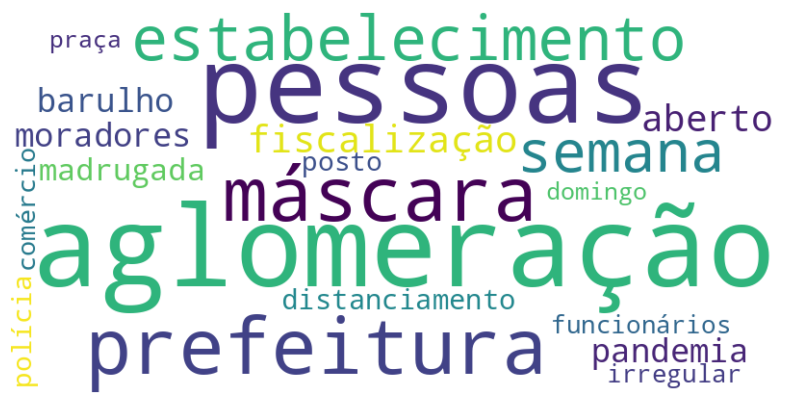
\includegraphics[width=0.7\textwidth]{images/wordcloud_social_distancing.png}
	\caption{Wordcloud com palavras mais frequentes em postagens sobre Distanciamento Social}
	\label{fig:wordcloud_social_distancing}
\end{figure}

A vigilância participativa, um conceito onde cidadãos contribuem ativamente para o monitoramento de questões de saúde pública, é evidenciada na maneira como os usuários do Colab relatam e reagem a situações relacionadas ao distanciamento social. A predominância de personas do tipo \textit{helper} em eventos como superlotação no transporte público mostra que os cidadãos não apenas identificam problemas, mas também estão dispostos a colaborar na busca de soluções ou demonstram uma certa empatia principalmente no que diz respeito ao distanciamento social em espaços de trânsito em massa. Este tipo de engajamento oferece às autoridades de saúde pública uma fonte valiosa de informações em tempo real, permitindo uma resposta mais rápida e eficiente a situações emergentes.

\begin{quadro}[htb]
	\centering
	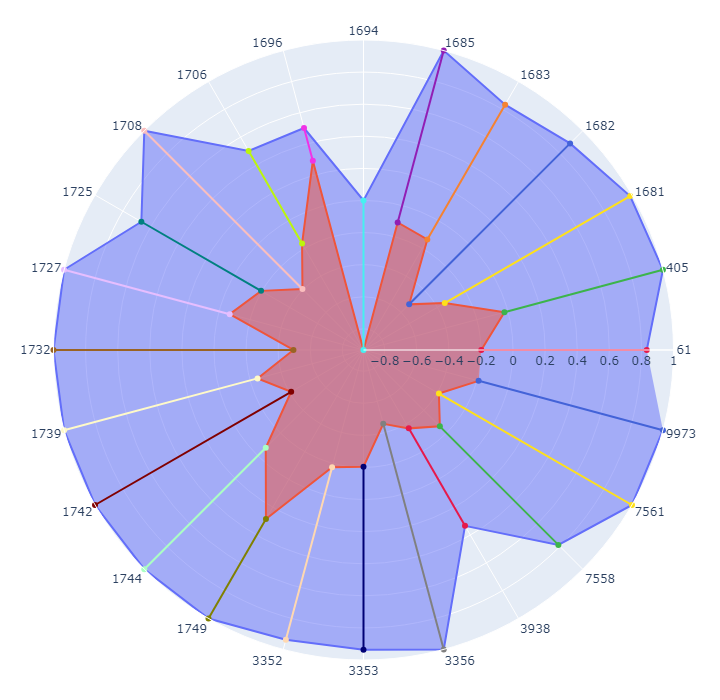
\includegraphics[width=0.7\textwidth]{images/social_barometer_social_distancing.png}
	\caption{Gráfico de Radar ilustrando a pressão social em relação ao tópico de Distanciamento Social.}
	\label{fig:social_barometer_social_distancing}
\end{quadro}

Por outro lado, a forte reação negativa em eventos como superlotação de ônibus e a predominância de personas do tipo \textit{complainer} indicam uma alta pressão social e insatisfação com a gestão atual desses problemas. Este feedback direto dos cidadãos é essencial para que as autoridades compreendam as áreas críticas que necessitam de atenção imediata e ajustem suas políticas e práticas em conformidade.

Além disso, a detecção digital de doenças, que envolve a utilização de dados digitais para monitorar e identificar tendências de saúde, é reforçada pela análise desses dados. A expressão de preocupações com aglomerações e condições sanitárias irregulares em estabelecimentos fornece às autoridades um panorama das preocupações de saúde em tempo real. Isso possibilita uma abordagem proativa na gestão de saúde pública, onde medidas preventivas e campanhas de conscientização podem ser direcionadas para áreas e temas específicos identificados através da plataforma.

Ao interpretar esses eventos sob a perspectiva de pressão social oferecemos uma nova dimensão para stakeholders, com o potencial aprimorar as estratégias de saúde pública, mas também capacitar uma resposta mais eficaz às preocupações emergentes, encorajando uma gestão colaborativa em crises de saúde. A interação ativa entre cidadãos e a análise crítica dessas informações estabelecem uma base para uma vigilância participativa eficiente e oferece oportunidades para estratégias de detecção digital de doenças. Essa abordagem não só reforça as medidas de saúde pública, mas também fortalece o bem-estar e a segurança da comunidade, demonstrando o poder da tecnologia e da participação cidadã na melhoria da saúde pública.

\subsection{Mudança Climática}
\label{sec:eventos_populares_weather}

\begin{figure}[htb]
	\centering
	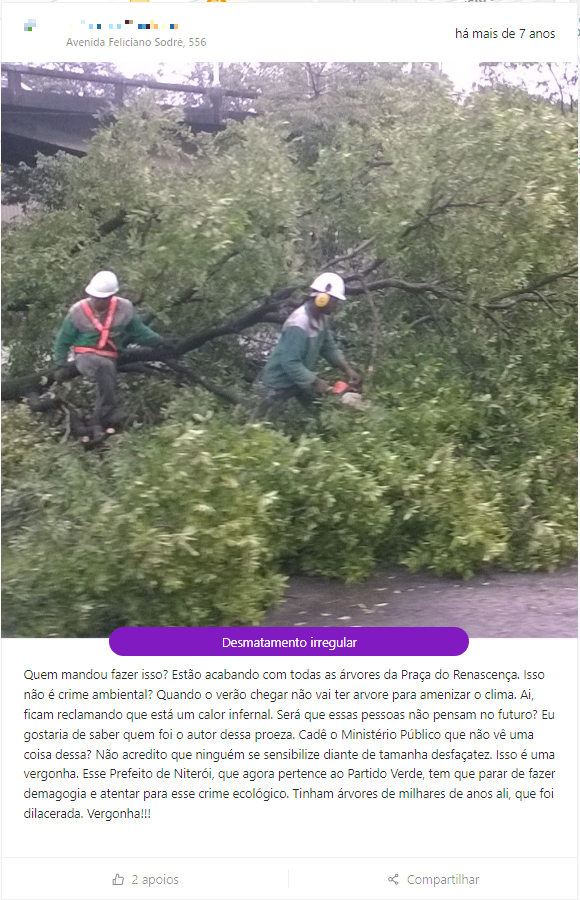
\includegraphics[width=0.7\textwidth]{images/colab_posts_social_clima.png}
	\caption{Exemplo de postagem no Colab denunciando os efeitos do desmatamento na mudança climática.}
	\label{fig:colab_posts_social_clima}
\end{figure}

Ao analisar os eventos do Colab, podemos filtrar por tipos de eventos e palavras-chave específicas ao tópico de mudanças climáticas, revelando como as preocupações cotidianas dos usuários em relação a problemas urbanos refletem uma consciência mais ampla sobre mudança climática. Esta abordagem permite identificar tendências e padrões específicos na percepção pública, ilustrando como as questões locais se entrelaçam com o debate global sobre o clima. Os dados refletem uma ampla variedade de reações a problemas urbanos e ambientais, desde a manutenção de espaços verdes até a gestão da infraestrutura urbana e questões de saúde pública. As métricas apresentadas na \autoref{tab:eventos_populares_weather} destacam a diversidade de eventos e a complexidade das opiniões dos cidadãos em relação às mudanças climáticas e meio ambiente, o que demonstra uma crescente sensibilidade a crises ambientais e a necessidade de ações proativas.

\begin{figure}[htb]
	\centering
	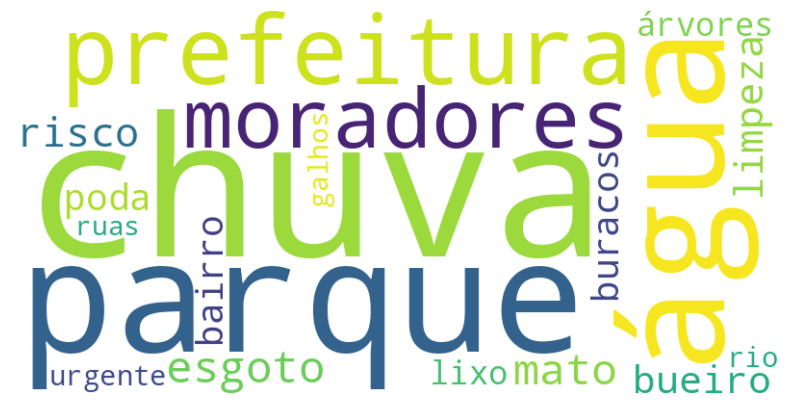
\includegraphics[width=0.7\textwidth]{images/wordcloud_weather.png}
	\caption{Wordcloud com palavras mais frequentes em postagens sobre Mudança Climática}
	\label{fig:wordcloud_weather}
\end{figure}

O interesse significativo da comunidade em eventos proativos, como iniciativas de arborização, apesar de uma participação ativa limitada, sugere um reconhecimento geral da importância de tais ações para a sustentabilidade ambiental. Por outro lado, a forte reação negativa e a postura crítica em relação a problemas como desmatamento irregular e ocupação de áreas públicas destacam uma preocupação profunda com a perda de espaços naturais e a preservação ambiental.

\begin{quadro}[htb]
	\centering
	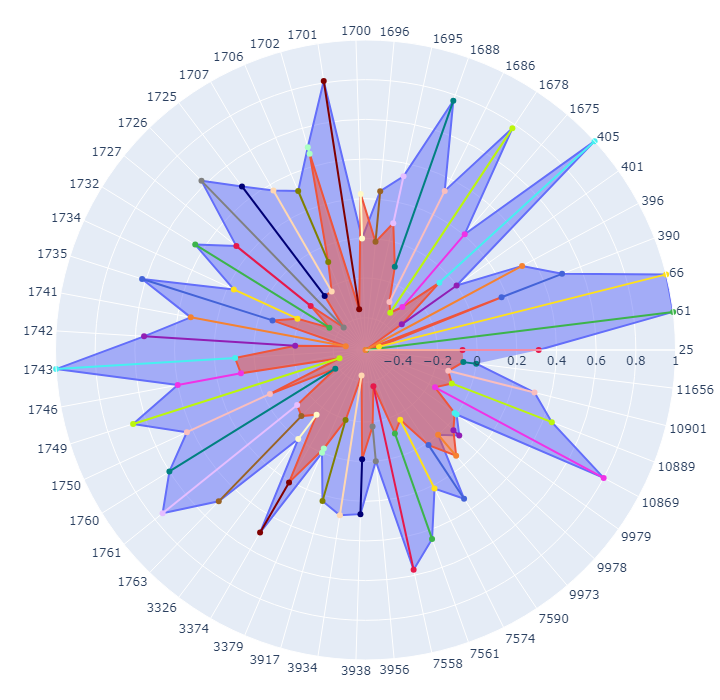
\includegraphics[width=0.7\textwidth]{images/social_barometer_weather.png}
	\caption{Gráfico de Radar ilustrando a pressão social em relação ao tópico de Mudança Climática.}
	\label{fig:social_barometer_weather}
\end{quadro}

A análise revela uma polarização nas atitudes em relação às mudanças climáticas. Alguns usuários criam eventos que diretamente vinculam as mudanças climáticas como a causa de problemas urbanos, enquanto outros abordam esses problemas como questões de gestão pública ou falta de ação por parte dos agentes governamentais. Essa polarização reflete as diferentes perspectivas dos usuários, onde alguns veem as mudanças climáticas como uma motivação subjacente para os problemas, enquanto outros focam nas questões de governança e gestão pública. Essa diversidade de abordagens pode ser vista como um reflexo das opiniões variadas dos usuários em relação às mudanças climáticas e à forma como elas se manifestam em suas comunidades.

Os resultados apontam para a necessidade de estratégias de comunicação e engajamento mais eficazes para abordar essa divisão. A compreensão dessas dinâmicas é crucial para os formuladores de políticas e gestores públicos, pois permite o desenvolvimento de abordagens mais inclusivas e abrangentes que considerem as diversas perspectivas e preocupações dos cidadãos. Esta análise destaca a importância de incorporar a voz da comunidade no planejamento e na implementação de políticas de mudança climática e gestão ambiental.

\subsection{Paisagismo}
\label{sec:eventos_populares_landscape}

\begin{figure}[htb]
	\centering
	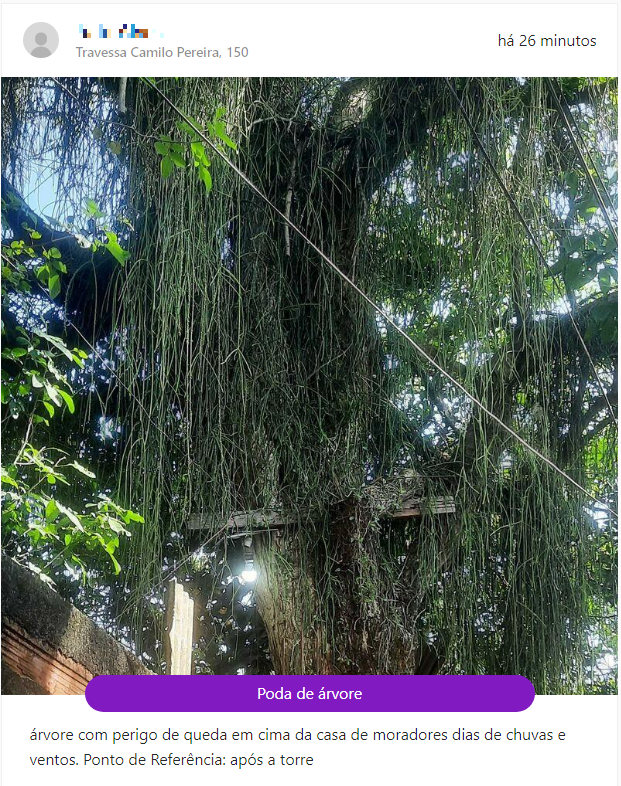
\includegraphics[width=0.7\textwidth]{images/colab_posts_paisagismo.png}
	\caption{Exemplo de postagens no Colab sobre Paisagismo}
	\label{fig:colab_posts_paisagismo}
\end{figure}

O paisagismo e como cidades tratam tópicos como arborização e o gerenciamento de parques e praças não se trata somente de uma preocupação estética; é um elemento intrínseco à qualidade de vida nas cidades, com repercussões significativas em áreas como meio ambiente, mudanças climáticas e no bem-estar da população. A análise dos dados de pressão social hiperlocal revela uma variedade de perspectivas e preocupações dos cidadãos em relação a eventos de paisagismo em suas comunidades. As métricas foram resumidas na \autoref{tab:eventos_populares_landscape} e demonstram que além de se preocuparem com o meio ambiente em um nível macro como alagamentos e ondas de calor, os usuários também estão preocupados com o seu ecossistema local, representado principalmente por demandas de paisagismo.

\begin{figure}[htb]
	\centering
	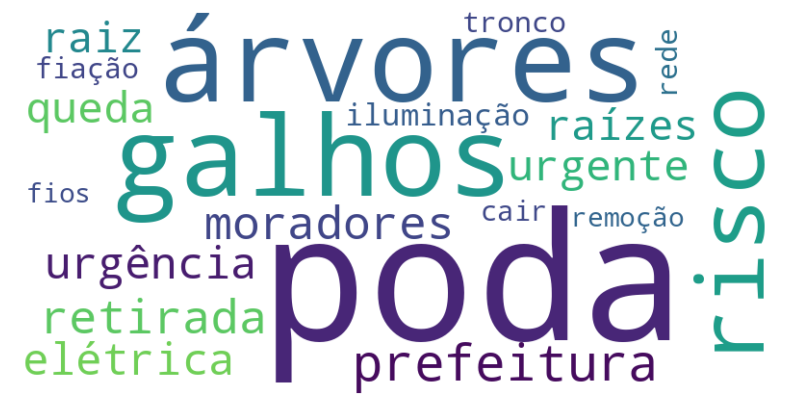
\includegraphics[width=0.7\textwidth]{images/wordcloud_landscape.png}
	\caption{Wordcloud com palavras mais frequentes em postagens sobre Paisagismo}
	\label{fig:wordcloud_landscape}
\end{figure}

A análise mostra que eventos como a poda de árvores e a retirada de árvores frequentemente geram um debate considerável. A persona associada a esses eventos varia, refletindo uma diversidade de opiniões. Enquanto alguns cidadãos expressam apoio às práticas de manejo da vegetação urbana, destacando a importância da segurança e estética, outros manifestam preocupações sobre o impacto na preservação das áreas verdes e sombra nas cidades. Isso demonstra a complexidade das questões relacionadas à vegetação urbana e destaca a necessidade de políticas e práticas que considerem essa diversidade de perspectivas.

\begin{quadro}[htb]
	\centering
	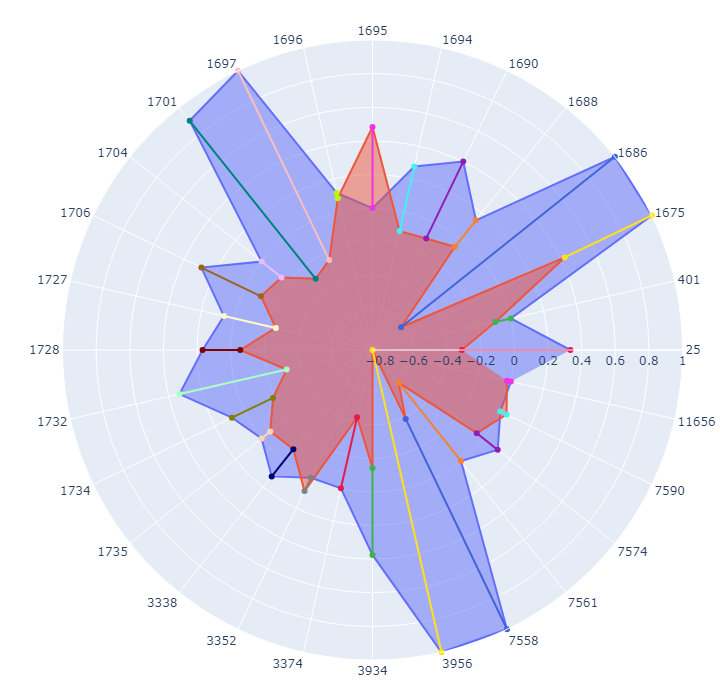
\includegraphics[width=0.7\textwidth]{images/social_barometer_landscape.png}
	\caption{Gráfico de Radar ilustrando a pressão social em relação ao tópico de Paisagismo}
	\label{fig:social_barometer_landscape}
\end{quadro}

Além disso, eventos como desmatamento irregular e equipamento público danificado recebem críticas significativas. Isso sugere que os cidadãos estão atentos à conservação das áreas verdes urbanas e à manutenção adequada de espaços públicos. Essas preocupações estão intrinsecamente ligadas à qualidade de vida nas cidades, pois afetam a acessibilidade, segurança e o uso desses espaços. Outros eventos, como a ocupação irregular de áreas públicas, demonstram uma persona predominantemente \textit{complainer}, indicando insatisfação com o uso inadequado de espaços urbanos. A falta de calçadas e faixas de pedestres em boas condições também gera críticas, evidenciando a importância da infraestrutura urbana para a mobilidade e segurança dos cidadãos.

A conexão entre paisagismo e questões ambientais, como mudanças climáticas, é evidente em eventos como a poda de árvores e a retirada de árvores. O manejo inadequado da vegetação urbana pode afetar a regulação da temperatura local e a absorção de poluentes, destacando a necessidade de práticas sustentáveis de paisagismo. No entanto, é importante notar que as árvores também podem ter um impacto no fornecimento de energia elétrica. Eventos relacionados à falta de energia e fiação irregular indicam a preocupação dos cidadãos com a confiabilidade da infraestrutura elétrica em espaços públicos. Árvores próximas a fios de energia podem representar um risco, evidenciando a necessidade de equilibrar a preservação da vegetação com a segurança energética.

A análise da pressão social do paisagismo urbano destaca a complexidade das questões envolvidas e a diversidade de perspectivas dos cidadãos. Isso ressalta a importância de uma abordagem aberta e inclusiva na gestão do paisagismo, considerando as expectativas e necessidades da comunidade. Além disso, a conexão entre paisagismo, meio ambiente, mudanças climáticas e energia elétrica destaca a necessidade de políticas e práticas que promovam a sustentabilidade e o bem-estar nas cidades.

\subsection{Meio Ambiente}
\label{sec:eventos_populares_environment}

\begin{figure}[htb]
	\centering
	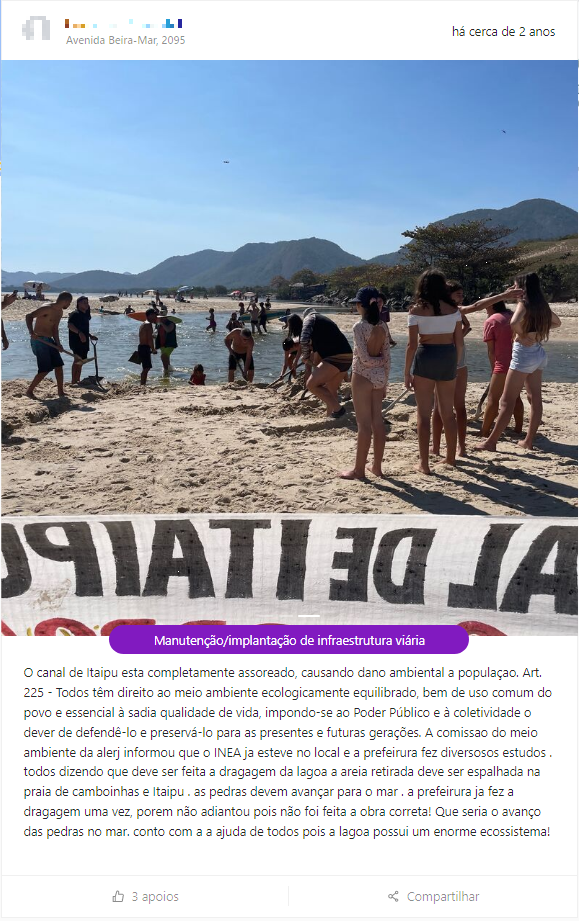
\includegraphics[width=0.7\textwidth]{images/colab_posts_social_environment.png}
	\caption{Postagem do colab evidenciando o engajamento cívico em questões ambientais.}
	\label{fig:colab_posts_social_environment}
\end{figure}

O meio ambiente é um tópico de extrema importância para as comunidades urbanas em todo o mundo, uma vez que as questões ambientais têm um impacto direto na qualidade de vida dos cidadãos nas cidades. Isso abrange aspectos como saúde pública, acesso a áreas verdes, qualidade do ar e da água, biodiversidade urbana e clima local. A qualidade do ambiente urbano influencia a saúde física e mental dos habitantes das cidades, sendo a poluição do ar, a contaminação da água e a falta de áreas verdes causadoras de problemas de saúde, como doenças respiratórias, alergias, doenças cardiovasculares e estresse. Além disso, a degradação ambiental pode afetar negativamente a economia das cidades, com desvalorização imobiliária e deslocamento de comunidades de baixa renda de áreas afetadas. A preservação de espaços verdes urbanos desempenha um papel importante na regulação do clima e na melhoria da qualidade do ar, e a sustentabilidade a longo prazo das cidades depende de práticas ambientalmente responsáveis, como reciclagem e eficiência energética.

\begin{figure}[htb]
	\centering
	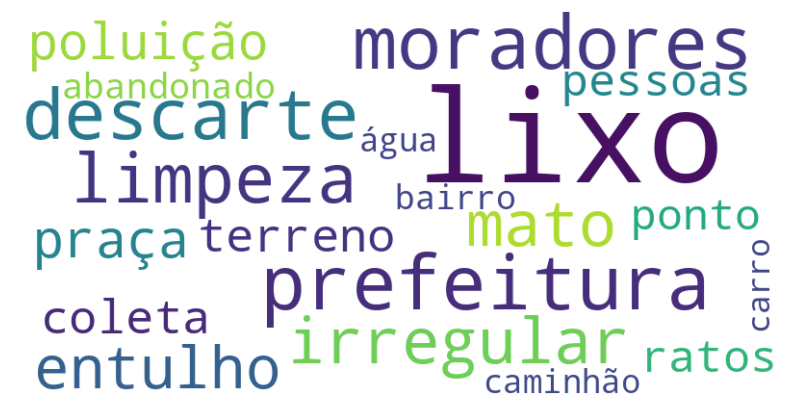
\includegraphics[width=0.7\textwidth]{images/wordcloud_environment.png}
	\caption{Wordcloud com palavras mais frequentes em postagens sobre Meio Ambiente}
	\label{fig:wordcloud_environment}
\end{figure}

\begin{quadro}[htb]
	\centering
	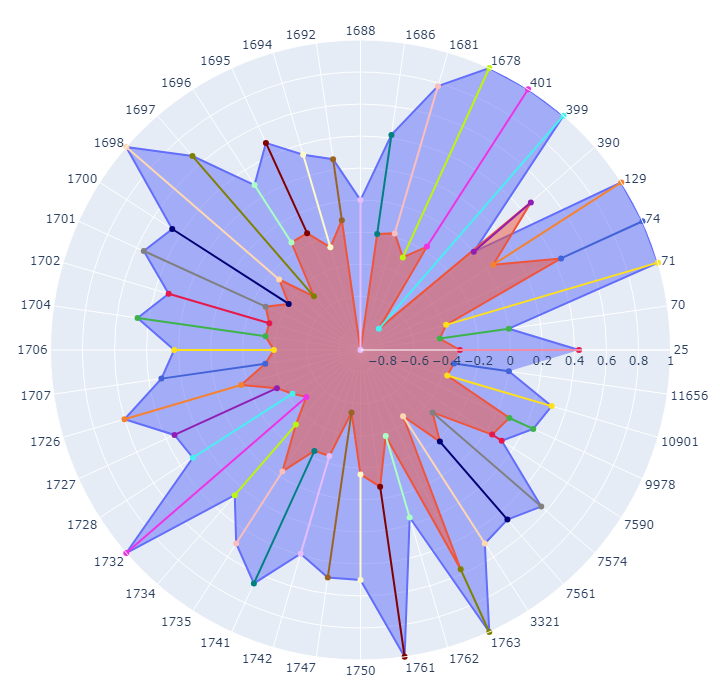
\includegraphics[width=0.7\textwidth]{images/social_barometer_environment.png}
	\caption{Gráfico de Radar ilustrando a pressão social em relação ao tópico de Meio Ambiente}
	\label{fig:social_barometer_environment}
\end{quadro}

Ao analisar as métricas de pressão social resumidas na \autoref{tab:eventos_populares_environment}, observamos uma intersecção de tipos de eventos comuns a crise climática e paisagismo. Em alguns tópicos, como proteção animal, a maioria dos usuários adota uma abordagem colaborativa e positiva, demonstrando preocupação com a fauna e o meio ambiente. No entanto, em eventos relacionados a questões de saneamento básico e conservação da água, os usuários tendem a expressar insatisfação e críticas, refletindo preocupações com problemas como coleta inadequada de lixo e esgoto a céu aberto. A participação ativa em discussões sobre questões de paisagismo e arborização indica um desejo de melhorar as áreas verdes urbanas. Em relação às mudanças climáticas, eventos como incêndios florestais e desmatamento ilegal recebem críticas, indicando preocupações com a degradação ambiental. Além disso, a popularidade de eventos relacionados ao saneamento básico e áreas verdes urbanas sugere que esses problemas são altamente relevantes para a qualidade de vida nas cidades e despertam o interesse dos usuários. No entanto, é importante observar que essas discussões frequentemente refletem insatisfação com os serviços públicos relacionados a esses eventos, destacando a necessidade de melhorias.

Os dados também podem ser utilizados pelos administradores das cidades para promover ações que melhorem a qualidade de vida dos habitantes urbanos e a sustentabilidade ambiental. Primeiramente, a compreensão da diversidade de perspectivas dos usuários em relação a questões ambientais permite que os administradores considerem uma ampla gama de opiniões ao tomar decisões relacionadas ao meio ambiente. Isso pode ajudar a evitar soluções unilaterais e a garantir que as políticas e iniciativas sejam mais abrangentes e eficazes. Por exemplo, ao lidar com problemas de saneamento básico, os administradores podem levar em consideração as críticas e insatisfações expressas pelos usuários e buscar soluções que atendam às suas preocupações.

Além disso, a popularidade de eventos relacionados a questões ambientais indica quais problemas são mais relevantes para a população urbana. Os administradores podem usar essas informações para priorizar recursos e esforços em áreas que afetam significativamente a qualidade de vida das pessoas. Por exemplo, se eventos relacionados ao descarte irregular de lixo são amplamente discutidos, isso pode sinalizar a necessidade de melhorias na coleta de resíduos e na conscientização ambiental. A análise das personas médias dos usuários em diferentes tópicos também é informativa. Por exemplo, em eventos relacionados à proteção animal, a predominância da persona \textit{helper} indica um desejo de colaboração e apoio a iniciativas de preservação da fauna. Os administradores podem aproveitar esse espírito colaborativo para envolver a comunidade em esforços de conservação da vida selvagem e educação ambiental.

Por outro lado, em eventos relacionados a problemas de saneamento básico, onde a persona \textit{complainer} é mais comum, os administradores podem reconhecer a necessidade de abordar preocupações específicas e melhorar os serviços relacionados. Isso pode incluir a implementação de sistemas de coleta de lixo mais eficientes ou ações para evitar o esgoto a céu aberto. Os administradores podem usar essas métricas para identificar oportunidades de melhoria em áreas como paisagismo urbano e mitigação das mudanças climáticas. Por exemplo, ao reconhecer a disposição dos usuários em participar de iniciativas de plantio de árvores, os administradores podem promover programas de arborização urbana que não apenas tornam a cidade mais verde, mas também envolvem a comunidade.

Em resumo, dessas métricas não se limita apenas a fornecer um panorama das opiniões dos usuários, mas também oferece orientações valiosas para os administradores das cidades. Esses dados podem ser usados para tomar decisões informadas, priorizar áreas de atuação e envolver a comunidade de maneira mais eficaz na promoção de um ambiente urbano saudável e sustentável. Portanto, ao compreender as perspectivas e preocupações dos cidadãos, os administradores podem implementar políticas e iniciativas que atendam melhor às necessidades da população e ao meio ambiente.

\subsection{Gentrificação}
\label{sec:eventos_populares_social_gentrification}

\begin{figure}[htb]
	\centering
	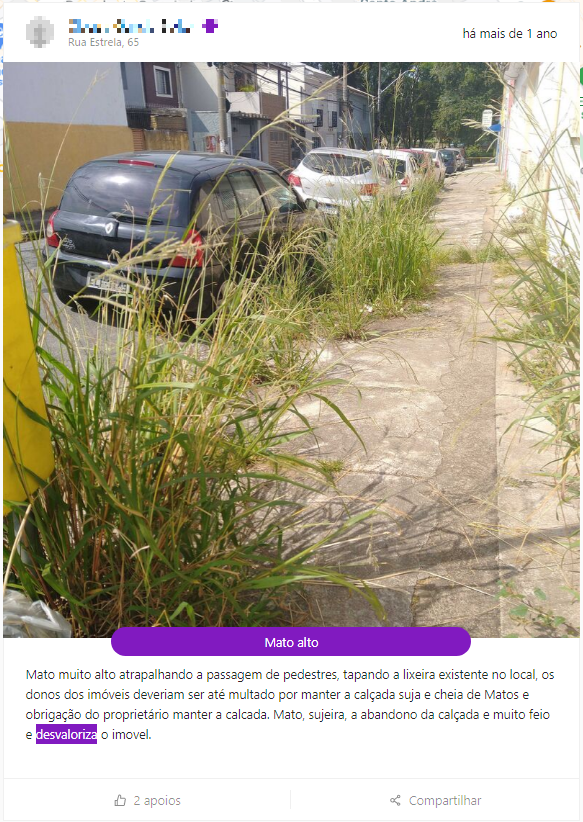
\includegraphics[width=0.7\textwidth]{images/colab_posts_social_gentrification.png}
	\caption{Usuário reclama da desvalorização de imóveis causada por mato alto.}
	\label{fig:colab_posts_social_gentrification}
\end{figure}

A gentrificação tem se consolidado como um dos tópicos mais debatidos nas discussões sobre desenvolvimento urbano, desencadeando paixões e preocupações de diferentes partes da população. Dada a sua natureza multidimensional, é imperativo entender as nuances de como a gentrificação é percebida e quais as principais áreas de preocupação. Através da análise de dados de postagens de eventos de zeladoria pública no Colab, podemos criar um tópico de pressão social que nos informa sobre a opinião e sentimento dos usuários apresentado na \autoref{tab:eventos_populares_social_gentrification}.

\begin{figure}[htb]
	\centering
	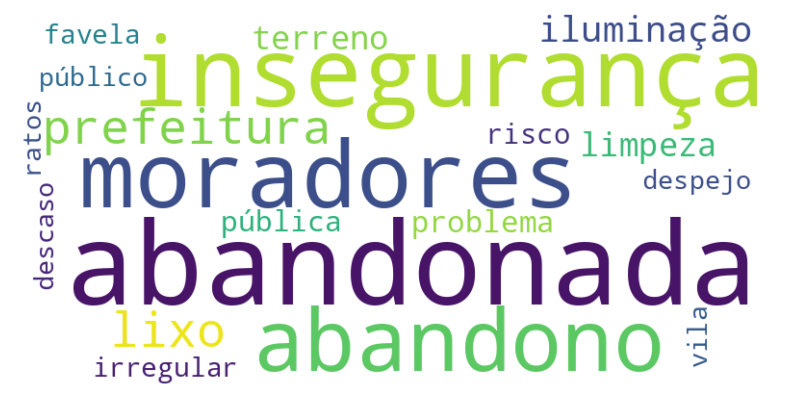
\includegraphics[width=0.7\textwidth]{images/wordcloud_gentrification.png}
	\caption{Wordcloud com palavras mais frequentes em postagens sobre Gentrificação}
	\label{fig:wordcloud_gentrification}
\end{figure}

\begin{quadro}[htb]
	\centering
	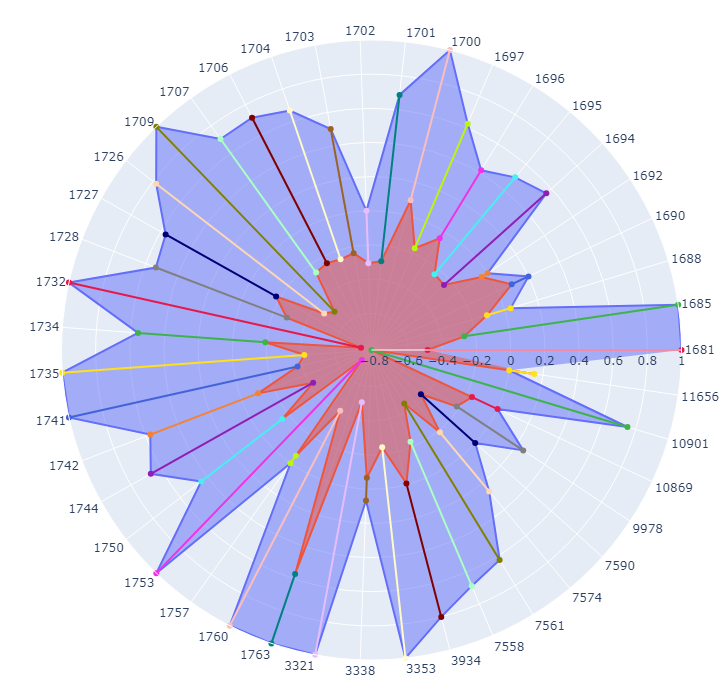
\includegraphics[width=0.7\textwidth]{images/social_barometer_gentrification.png}
	\caption{Gráfico de Radar ilustrando a pressão social em relação ao tópico de Gentrificação}
	\label{fig:social_barometer_gentrification}
\end{quadro}

Os dados revelam uma polarização entre dois grupos de usuários: aqueles que têm interesses econômicos na área, como proprietários de imóveis, que reportam eventos relacionados à desvalorização da propriedade; e aqueles preocupados com os impactos adversos da gentrificação, como despejos, que reportam eventos indicando uma degradação das condições de vida e do acesso a espaços públicos.

Os sentimentos expressos nas postagens também variam, com eventos relacionados à poluição sonora e desmatamento tendo sentimentos predominantemente negativos, enquanto eventos sobre parques e praças recebem avaliações mais positivas. A persona média tende a se inclinar para a categoria \textit{complainer} em muitos tópicos, indicando insatisfação e demanda por melhorias.

\begin{figure}[htb]
	\centering
	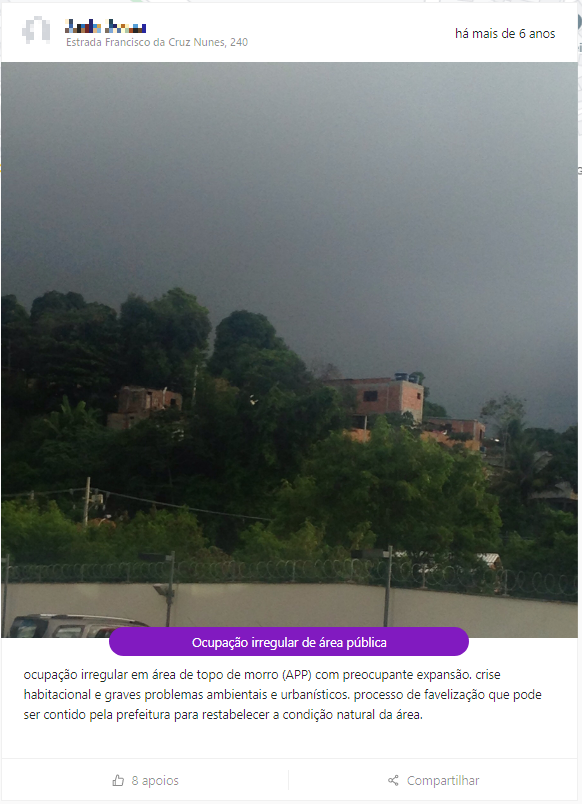
\includegraphics[width=0.7\textwidth]{images/colab_posts_social_favelizacao.png}
	\caption{Usuário denuncia ocupaçao irregular de área pública e aluz a favelização.}
	\label{fig:colab_posts_social_favelizacao}
\end{figure}

Os eventos mais populares, como o descarte irregular de lixo e imóveis abandonados, refletem a preocupação com a degradação e falta de zeladoria, sugerindo que a gentrificação não se limita à chegada de novos moradores, mas também envolve negligência e abandono de áreas valorizadas anteriormente.

Os dados revelam tendências importantes, como a crescente preocupação com a insegurança e deterioração das áreas afetadas pela gentrificação, bem como a expulsão de moradores de longa data devido à especulação imobiliária. Além disso, há consciência sobre os fatores econômicos por trás da gentrificação, como especulação imobiliária e privatização.

Essa análise pode ser valiosa para os administradores das cidades ao informar políticas públicas relacionadas à gentrificação. Os dados destacam a necessidade de abordagens equilibradas que considerem tanto o desenvolvimento econômico quanto o bem-estar das comunidades. Políticas que promovam a inclusão, a preservação do patrimônio cultural e a melhoria da infraestrutura podem ajudar a minimizar os efeitos negativos da gentrificação e promover um desenvolvimento urbano mais sustentável.

\subsection{Higienismo Urbano}
\label{sec:eventos_populares_homeland}

\begin{figure}[htb]
	\centering
	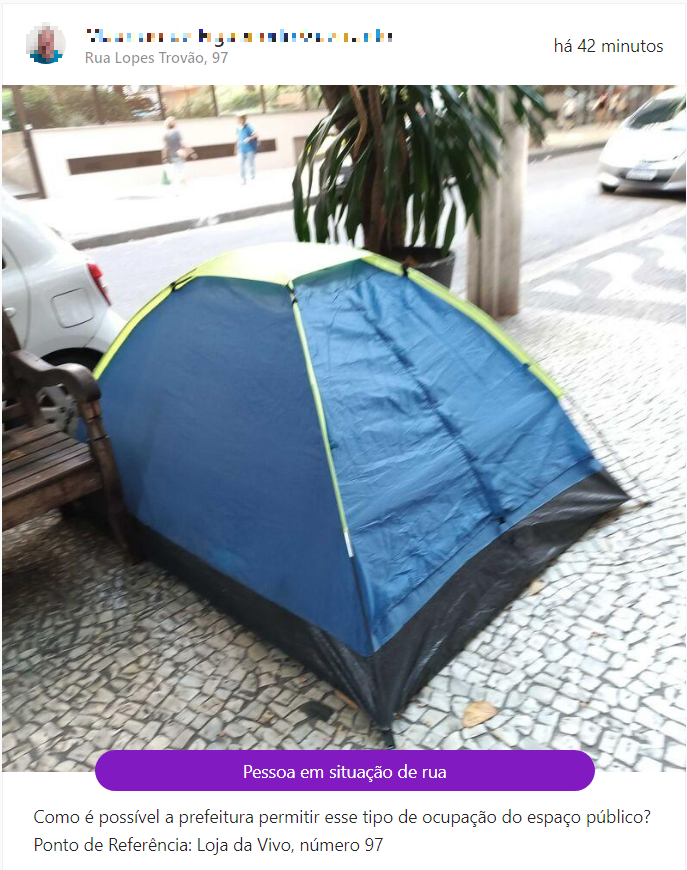
\includegraphics[width=0.7\textwidth]{images/colab_posts_higienismo.png}
	\caption{Exemplo de postagens sobre Higienismo Urbano no Colab}
	\label{fig:colab_posts_higienismo}
\end{figure}

Higienismo urbano é um tópico complexo que se relaciona com a maneira como as cidades são projetadas e gerenciadas em busca de uma aparência 'limpa' e 'ordenada'. Em um exame mais profundo do termo, o higienismo urbano é entrelaçado com questões de exclusão e marginalização social. Historicamente, o higienismo foi uma abordagem nas cidades que buscava combater doenças e promover a salubridade por meio da construção de infraestruturas de saneamento e reordenamento urbano. No entanto, em tempos modernos, essa abordagem se estendeu além de questões puramente sanitárias e evoluiu para a promoção de cidades esteticamente agradáveis, muitas vezes à custa de deslocar ou invisibilizar populações vulneráveis.

O higienismo urbano refere-se a práticas e políticas que buscam 'limpar' ou 'embelezar' espaços urbanos através da remoção ou ocultação de populações e condições consideradas 'indesejadas'. Um exemplo notório dessa prática ocorreu durante os preparativos para a Copa do Mundo de 2014 no Brasil. No Rio de Janeiro, para apresentar uma imagem mais 'limpa' aos visitantes internacionais, algumas favelas localizadas em pontos estratégicos como às margens das vias expressas, foram ocultadas por tapumes. Esta tentativa de mascarar a realidade socioeconômica da cidade atraiu críticas significativas, pois, em vez de resolver as questões subjacentes, a medida apenas escondia o problema. Paralelamente, uma das manifestações mais tangíveis do higienismo urbano é o que se convencionou chamar de 'design hostil'. Esta prática arquitetônica visa tornar os espaços públicos intencionalmente desconfortáveis para deter certos grupos, especialmente os sem-teto. Bancos com divisórias que impedem o repouso e picos no chão para desencorajar que se deitem são exemplos comuns dessa abordagem. Ambas as práticas, seja o ocultamento das realidades urbanas ou o design hostil, refletem uma abordagem que prioriza a estética e a ordem em detrimento do bem-estar e dos direitos dos cidadãos.

\begin{figure}[htb]
	\centering
	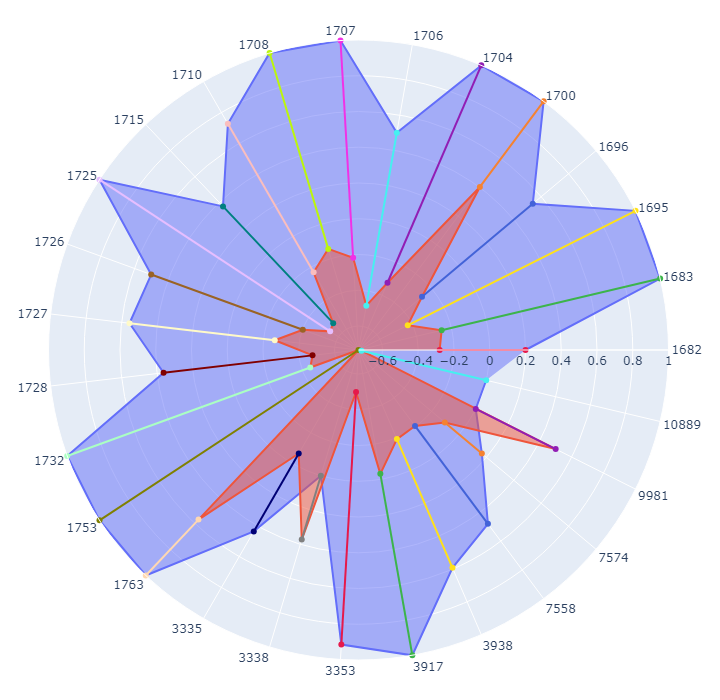
\includegraphics[width=0.7\textwidth]{images/social_barometer_homeland.png}
	\caption{Gráfico de Radar ilustrando a pressão social em relação ao tópico de Higienismo Urbano}
	\label{fig:social_barometer_homeland}
\end{figure}

O debate sobre o higienismo urbano revela uma polarização marcante. Por um lado, existem aqueles que apoiam ações de 'limpeza' e 'ordem' nas cidades, muitas vezes com uma perspectiva higienista. Por outro lado, há vozes que buscam abordagens mais humanas e inclusivas, procurando soluções reais para problemas sociais em vez de escondê-los ou afastá-los.

Os dados apresentados na \autoref{tab:eventos_populares_homeland} revelam essa divisão. Alguns eventos são percebidos como problemas por aqueles que têm uma atitude mais crítica, enquanto outros são vistos de forma positiva, refletindo o valor atribuído a espaços públicos bem conservados e serviços eficientes.

A polarização também se reflete na linguagem usada pelos usuários. Enquanto alguns expressam empatia ao mencionar 'moradores de rua', outros usam termos pejorativos, indicando a dicotomia na percepção pública. No entanto, há uma preocupação genuína com as populações vulneráveis, visto que problemas como 'Calçada inexistente' e 'Iluminação pública irregular' afetam a segurança e a acessibilidade de todos os cidadãos, especialmente os mais vulneráveis.

\begin{figure}[htb]
	\centering
	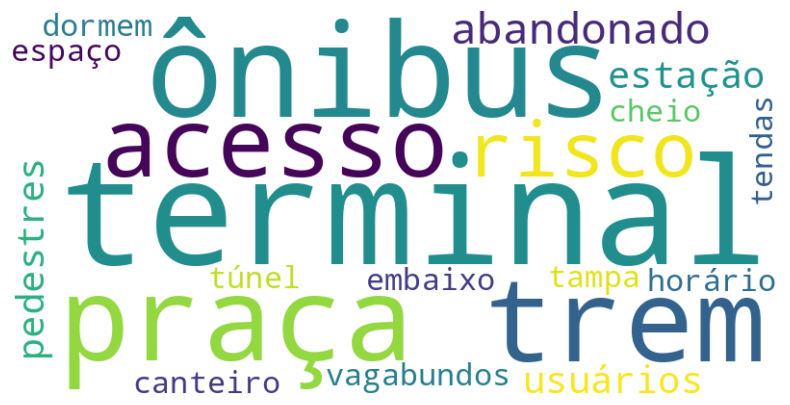
\includegraphics[width=0.7\textwidth]{images/wordcloud_homepand.png}
	\caption{Wordcloud com palavras mais frequentes em postagens sobre Higienismo Urbano}
	\label{fig:wordcloud_homepand}
\end{figure}

A dicotomia nos resultados demonstra um desafio para as cidades modernas: equilibrar o desejo por ordem e estética com a necessidade de justiça social e inclusão. O higienismo urbano e o design hostil são duas faces dessa moeda, e o conteúdo gerado por usuários de aplicativos como o Colab oferecem um vislumbre das opiniões e preocupações do público a respeito dessas questões.

Esses dados podem informar políticas públicas ao destacar a necessidade de um equilíbrio entre a busca por uma cidade mais ordenada e esteticamente agradável e a garantia de justiça social e inclusão. Administradores de cidades podem usar essas informações para desenvolver estratégias que abordem as preocupações legítimas dos cidadãos, ao mesmo tempo em que promovem a igualdade e o bem-estar de todos.

\subsection{Segurança Pública}
\label{sec:eventos_populares_security}

\begin{figure}[htb]
	\centering
	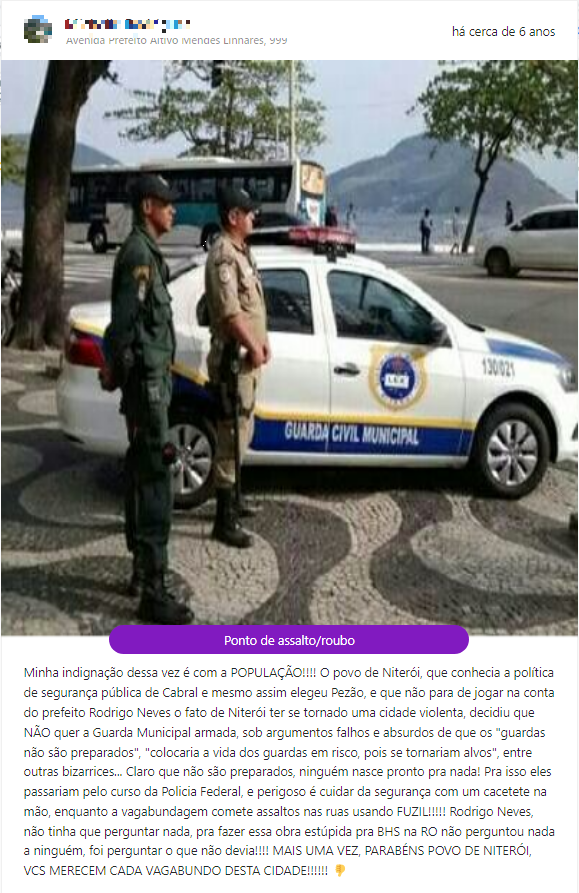
\includegraphics[width=0.7\textwidth]{images/colab_posts_security.png}
	\caption{Exemplo de um evento do Colab denunciando as inseguranças sentidas pelo usuário.}
	\label{fig:colab_posts_security}
\end{figure}

O cenário urbano brasileiro passou por transformações nas últimas décadas, especialmente na área de segurança pública, um tópico sensível e debatido. Nesse contexto, surgiram polarizações, principalmente entre defensores de abordagens repressivas e apoiadores de políticas sociais. Essas divisões muitas vezes refletem as inclinações políticas dos indivíduos e são amplificadas por líderes políticos e mídia.

\begin{figure}[htb]
	\centering
	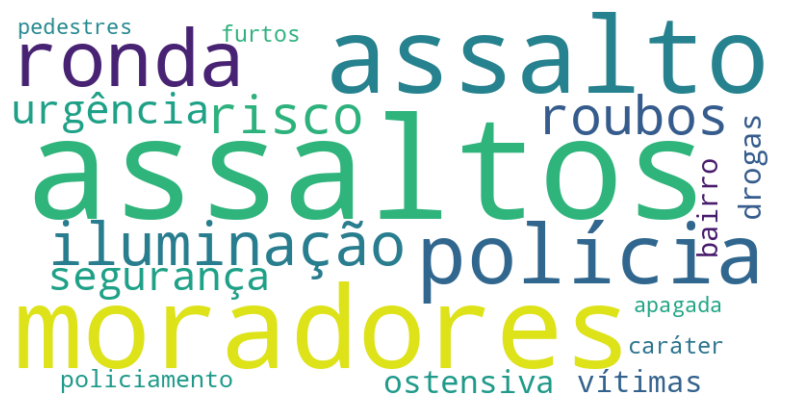
\includegraphics[width=0.7\textwidth]{images/wordcloud_security.png}
	\caption{Wordcloud com palavras mais frequentes em postagens sobre Segurança Pública}
	\label{fig:wordcloud_security}
\end{figure}

A alta incidência de assaltos e roubos, juntamente com um tom predominantemente negativo nas discussões, reflete uma preocupação significativa com a criminalidade. No entanto, a presença de ajudantes é menos notável, indicando que esses problemas podem ser vistos como desafiadores demais para ações comunitárias, exigindo intervenção governamental.

\begin{quadro}[htb]
	\centering
	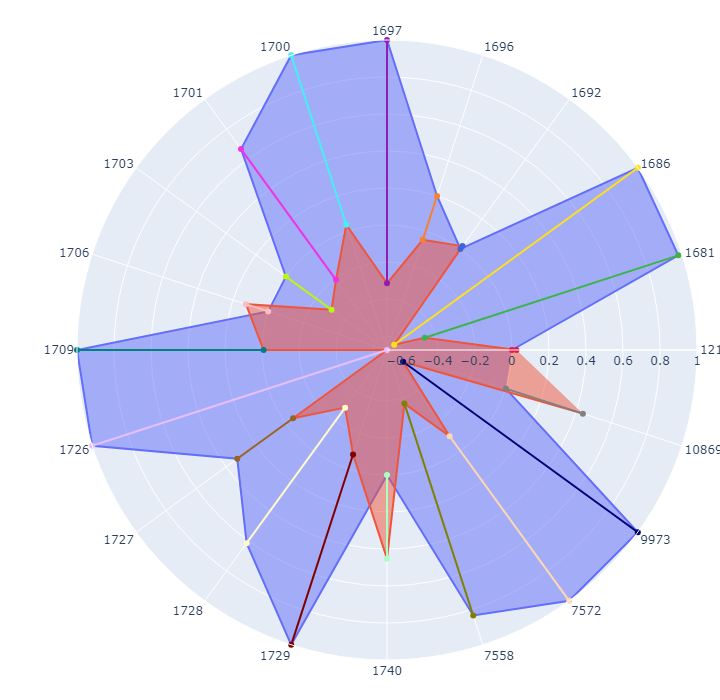
\includegraphics[width=0.7\textwidth]{images/social_barometer_security.png}
	\caption{Gráfico de Radar ilustrando a pressão social em relação ao tópico de Segurança Pública.}
	\label{fig:social_barometer_security}
\end{quadro}

A análise dos sentimentos e personas revela padrões interessantes. A \autoref{tab:eventos_populares_security} demonstra que eventos relacionados à poluição sonora e maus tratos a animais geram sentimentos negativos e são associados principalmente à persona \textit{complainer}. Por outro lado, eventos como vandalismo em bicicletários recebem reações positivas, sugerindo um engajamento positivo da comunidade.

No que diz respeito ao patrimônio público, há uma forte preocupação com a preservação do patrimônio histórico, refletida por uma alta incidência de personas \textit{complainer}. Isso destaca a valorização cultural e histórica da comunidade. No entanto, problemas estéticos, como pintura, geram reações menos intensas.

A análise revela uma polarização significativa na discussão sobre segurança pública, com predominância de reclamações e críticas. No entanto, também mostra um grupo ativo disposto a colaborar na identificação de soluções, principalmente para crimes contra a estrutura pública e a vida.

Esses dados indicam uma oportunidade para as autoridades locais capitalizarem o engajamento ativo da comunidade, direcionando-o para iniciativas colaborativas de segurança e melhorias urbanas. No entanto, também representam um desafio em termos de gestão e resposta às expectativas dos cidadãos, exigindo uma abordagem equilibrada que inclua todas as vozes da comunidade em um diálogo construtivo. Essas informações podem ser valiosas para informar políticas públicas relacionadas à segurança pública nas cidades.

A conclusão que emerge desses dados é a de uma comunidade ativamente engajada nas questões de segurança pública, mas cujo engajamento é predominantemente orientado para a expressão de preocupações e demandas por ação. Isso sinaliza uma oportunidade para os tomadores de decisão e as autoridades locais de capitalizar sobre essa participação ativa, canalizando-a para iniciativas colaborativas de segurança e melhorias urbanas. Ao mesmo tempo, revela um desafio significativo em termos de gestão e resposta às expectativas dos cidadãos, exigindo uma abordagem que equilibre a resposta imediata às preocupações com a promoção de um diálogo construtivo que inclua todas as vozes da comunidade.

\subsection{Política de Drogas}
\label{sec:eventos_populares_drugs}

\begin{figure}[htb]
	\centering
	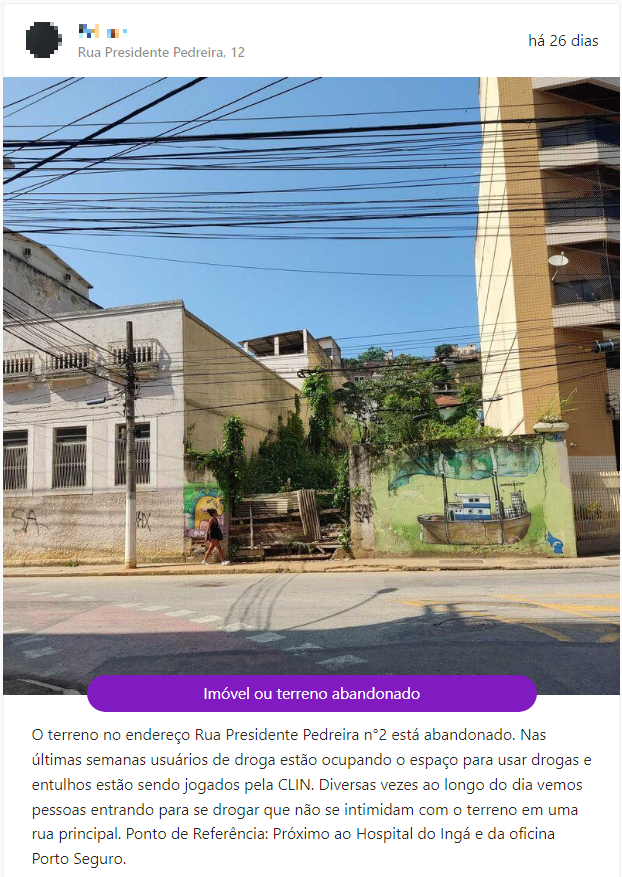
\includegraphics[width=0.7\textwidth]{images/colab_posts_drugs.png}
	\caption{Exemplo de postagem de um usuário denunciando um terreno abandonado usado para consumo de drogas.}
	\label{fig:colab_posts_drugs}
\end{figure}

A questão das drogas nas cidades do Brasil é complexa e abrange diversos aspectos, como saúde pública, segurança e questões sociais, econômicas e políticas. A política de drogas gera polarização, com diferentes perspectivas, desde abordagens mais focadas na prevenção e tratamento até políticas mais rígidas de repressão. As métricas de pressão social sobre o tema disponíveis na \autoref{tab:eventos_populares_drugs} não possui tantos eventos quantos outros tópicos, mas ainda podem iluminar o discurso sobre drogas no Colab principalmente ao analisarmos o sentimento das postagens.

\begin{figure}[htb]
	\centering
	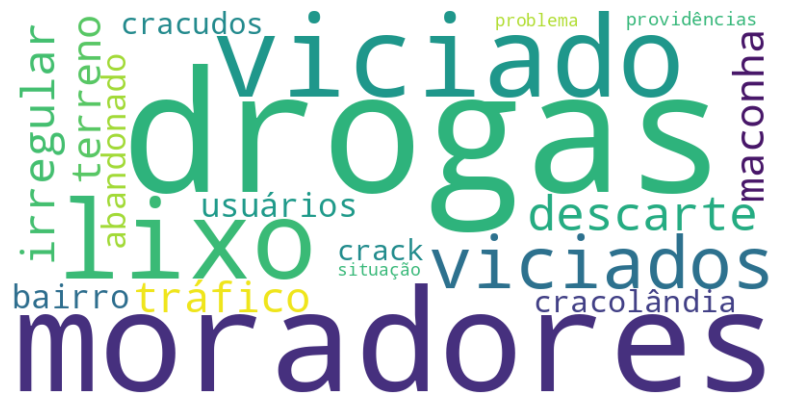
\includegraphics[width=0.7\textwidth]{images/wordcloud_drugs.png}
	\caption{Wordcloud com palavras mais frequentes em postagens sobre Política de Drogas}
	\label{fig:wordcloud_drugs}
\end{figure}

Ao analisar como os usuários do aplicativo Colab percebem o problema das drogas, observamos essa polarização. Alguns veêm o uso de drogas como um problema de saúde pública, destacando a necessidade de tratamento e apoio aos dependentes químicos. Outros o enxergam mais como uma questão de segurança pública, associando-o à criminalidade e degradação urbana. A forma como os usuários do Colab se referem aos usuários de drogas também revela essa polarização, com palavras negativas e estigmatizantes sendo usadas. Isso pode refletir uma tendência de responsabilizar o indivíduo pelo uso de drogas, em vez de considerar o contexto social e econômico mais amplo.

\begin{quadro}[htb]
	\centering
	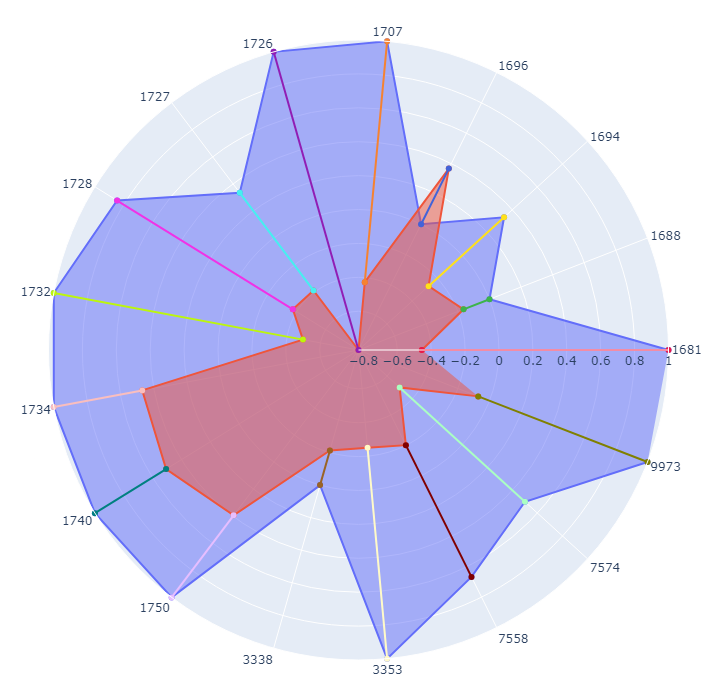
\includegraphics[width=0.7\textwidth]{images/social_barometer_drugs.png}
	\caption{Gráfico de Radar ilustrando a pressão social em relação ao tópico de Política de Drogas.}
	\label{fig:social_barometer_drugs}
\end{quadro}

Há também uma associação entre problemas de zeladoria pública e menções a drogas, sugerindo que áreas abandonadas ou negligenciadas podem se tornar locais propícios para o consumo e tráfico de drogas. Essa dinâmica destaca a necessidade de uma abordagem holística na gestão urbana, que não apenas aborde o problema das drogas, mas também as condições sociais e urbanas que o favorecem.

Para os administradores das cidades, esses dados podem ser valiosos na formulação de políticas públicas relacionadas às drogas. Eles devem considerar a necessidade de abordagens que abrangem tanto questões de saúde pública quanto de segurança, bem como investimentos em infraestrutura e revitalização de áreas degradadas. Uma abordagem integrada que leve em conta as percepções e experiências dos cidadãos, juntamente com os fatores estruturais e sociais é essencial para enfrentar o problema das drogas nas cidades.

\subsection{Pânico Moral}
\label{sec:eventos_populares_moral_panic}

\begin{figure}[htb]
	\centering
	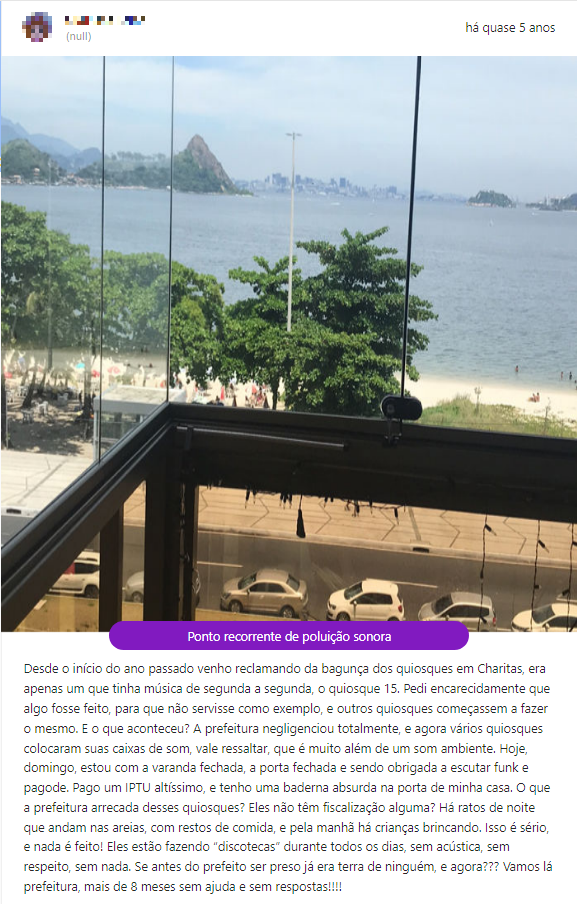
\includegraphics[width=0.7\textwidth]{images/colab_posts_karen.png}
	\caption{Exemplo de postagem de um usuário denunciando um evento de poluição sonora e associando-o a um gênero musical.}
	\label{fig:colab_posts_karen}
\end{figure}

O conceito de 'pânico moral', conforme delineado por Stanley Cohen em sua obra seminal 'Folk Devils and Moral Panics', fornece um quadro interpretativo valioso para compreender como certas questões sociais e comportamentos são amplificados e distorcidos dentro do discurso público, levando à criação de 'bodes expiatórios' ou 'demônios sociais'. No contexto brasileiro contemporâneo, e especialmente através de plataformas interativas como o Colab, podemos observar a manifestação desse fenômeno de forma peculiar. Cohen descreve o pânico moral como uma reação da sociedade a um grupo ou subcultura percebida como ameaçadora aos valores e interesses sociais estabelecidos \cite{2002_Cohen_BOOK}. Essa dinâmica é frequentemente caracterizada por uma distorção e exagero na percepção da ameaça. No Colab, essas expressões de pânico moral podem ser particularmente reveladoras, proporcionando uma janela para entender como certas preocupações são moldadas e amplificadas no espaço digital. Os dados da \autoref{tab:eventos_populares_moral_panic} apesar de limitados em quantidade, podem iluminar um pouco sobre o discurso dos usuários principalmente relacionados a certos tipos de demandas. 

Por exemplo, reclamações sobre poluição sonora, especialmente relacionadas a gêneros musicais como o funk e o pagode, podem refletir não apenas preocupações legítimas com o ruído, mas também preconceitos culturais e sociais. Isso se alinha com a noção de Cohen sobre a criação de 'bodes expiatórios', onde determinados estilos musicais e seus apreciadores são estigmatizados, representando mais do que uma mera perturbação sonora, mas sim uma ameaça à ordem e aos valores sociais.

\begin{figure}[htb]
	\centering
	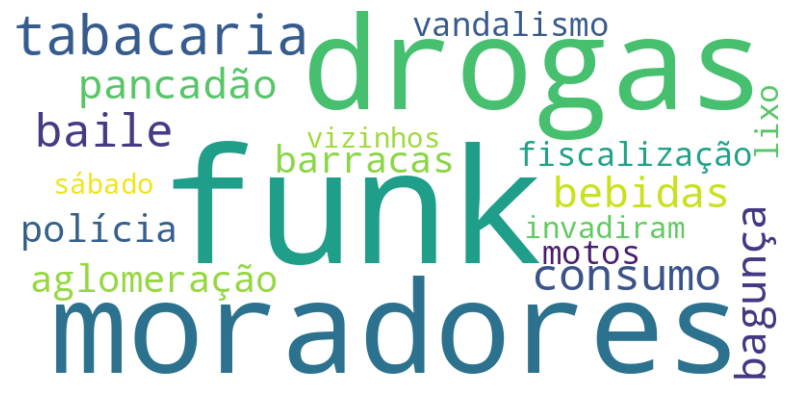
\includegraphics[width=0.7\textwidth]{images/wordcloud_moral.png}
	\caption{Wordcloud com palavras mais frequentes em postagens sobre Pânico Moral}
	\label{fig:wordcloud_moral}
\end{figure}

Além disso, o uso de termos pejorativos e discriminatórios em postagens relativas a eventos de zeladoria pública ou questões LGBTQIA+ pode sinalizar a presença de um pânico moral. Nesse contexto, grupos ou comportamentos são retratados de maneira distorcida, contribuindo para a disseminação de estereótipos e a marginalização de minorias. A presença de tais termos no Colab sugere que essas atitudes não estão restritas a esferas privadas ou conversas informais, mas se infiltram em discussões públicas sobre a gestão urbana e social.

A análise desses padrões de comunicação no Colab pode fornecer insights valiosos sobre as tensões subjacentes na sociedade brasileira. Permite aos pesquisadores e formuladores de políticas entender melhor não apenas as preocupações práticas dos cidadãos, mas também as dinâmicas psicossociais e culturais que moldam a percepção pública de certos grupos e questões. Ao identificar e analisar manifestações de pânico moral na plataforma, é possível adotar uma abordagem mais informada e matizada para enfrentar tanto as questões práticas da vida urbana quanto os desafios mais amplos de integração social e tolerância.

Ao analisar os resultados de pressão social, encontramos evidências claras de uma polarização relacionada à música, especialmente ao pagode e ao funk. Essa polarização é evidenciada pelos eventos de 'Ponto recorrente de poluição sonora' e 'Emissão de fumaça preta'. Ambos os eventos têm uma persona média predominantemente \textit{complainer}. Isso sugere que os usuários tendem a adotar uma abordagem crítica e insatisfeita em relação a eventos de poluição sonora, possivelmente devido ao impacto negativo do barulho, que frequentemente está associado a festas de pagode e funk. Essa conexão entre música e eventos de zeladoria pública demonstra um claro preconceito musical e uma polarização em relação a esses gêneros, que são percebidos negativamente por alguns membros da comunidade.

\begin{figure}[htb]
	\centering
	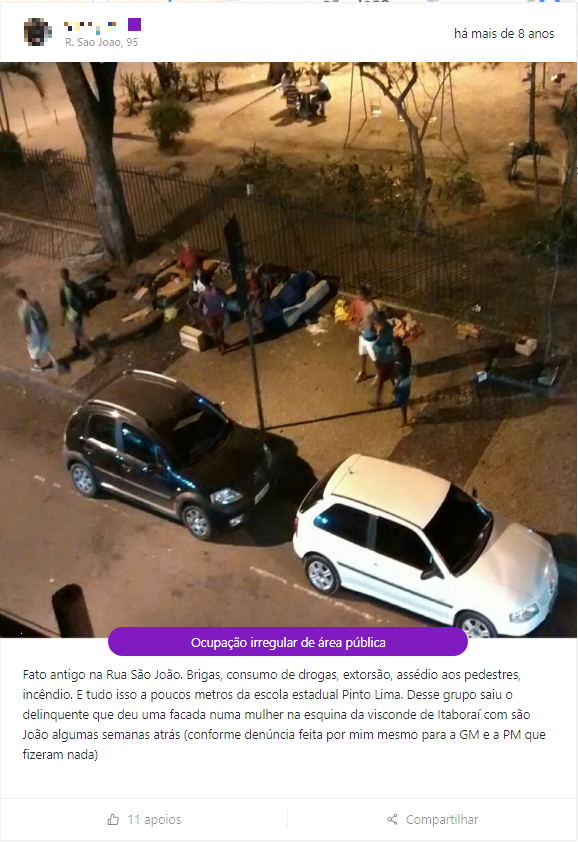
\includegraphics[width=0.7\textwidth]{images/colab_posts_moral_panic.png}
	\caption{Usuário denuncia ocupação irregular de área pública como degeneração urbana.}
	\label{fig:colab_posts_moral_panic}
\end{figure}

Além disso, as palavras-chave identificadas, como 'narguile', 'tabacaria' e 'grafite', sugerem que os usuários também estão associando comportamentos como fumar narguilé e grafites a eventos de zeladoria pública. Essas associações parecem ser negativas, pois esses eventos têm persona média predominantemente \textit{complainer}, refletindo a preocupação ou descontentamento dos usuários em relação a esses comportamentos. Essa conexão entre eventos culturais e preocupações com a zeladoria pública indica que a plataforma está sendo usada para expressar opiniões e críticas sobre questões culturais e comportamentais, além das questões de infraestrutura tradicionais.

Outro aspecto importante a ser destacado é a associação entre eventos de zeladoria pública, como 'Fiação irregular', 'Ocupação irregular de área pública' e 'Construção irregular', e os eventos culturais mencionados anteriormente, como bailes de funk e pagode. Os usuários parecem se incomodar com o barulho e a informalidade desses eventos e, como resultado, criam eventos de zeladoria pública para relatar irregularidades e tentar fechar esses estabelecimentos. Essa estratégia sugere uma tentativa de utilizar as ferramentas disponíveis na plataforma para influenciar o fechamento desses locais, refletindo uma tentativa de impor normas sociais e urbanas.

\begin{quadro}[htb]
	\centering
	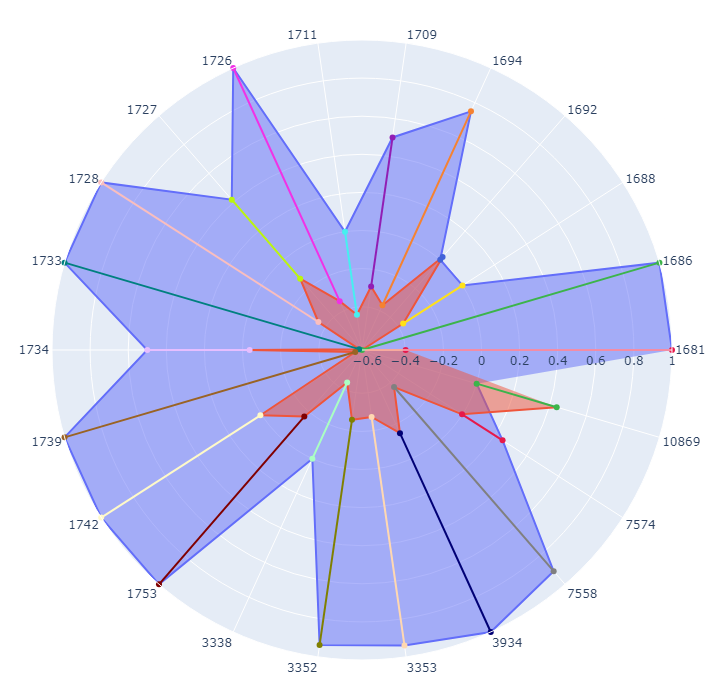
\includegraphics[width=0.7\textwidth]{images/social_barometer_moral.png}
	\caption{Gráfico de Radar ilustrando a pressão social em relação ao tópico de Pânico Moral.}
	\label{fig:social_barometer_moral}
\end{quadro}

A associação entre eventos culturais e eventos de zeladoria pública também é evidente nas métricas de pressão social. Os eventos de 'Comércio aberto irregularmente', 'Aglomeração de pessoas' e 'Evento Irregular' têm persona média equilibrada entre \textit{helper} e \textit{complainers}. Isso indica uma diversidade de opiniões em relação a esses eventos, possivelmente refletindo a complexidade do tópico e as diferentes perspectivas dos usuários. Essa diversidade sugere que, enquanto alguns usuários estão preocupados com a infração das regras e o impacto negativo na comunidade, outros podem ver esses eventos como oportunidades culturais ou econômicas.

Além disso, a questão da informalidade na organização desses eventos culturais, como mencionado com bailes de funk e pagode, é uma preocupação subjacente. Os eventos de 'Imóvel ou terreno abandonado' e 'Patrimônio histórico em risco' também refletem uma persona média predominantemente \textit{complainer}. Isso sugere que os usuários frequentemente expressam insatisfação em relação à falta de preservação do patrimônio histórico e à presença de imóveis ou terrenos abandonados, possivelmente relacionando essas questões à informalidade e ao descuido urbanos.

No entanto, é importante notar que, apesar da polarização evidente em relação a eventos culturais e comportamentais, outros eventos, como 'Lixeira quebrada', 'Descarte irregular de lixo' e 'Poda de árvore', têm persona média mais equilibrada, sugerindo que os usuários tendem a adotar uma postura mais colaborativa e positiva em relação a essas questões de infraestrutura.

Em relação à questão da polarização, os resultados indicam que a música, especialmente os gêneros de pagode e funk, parece ser um ponto sensível que gera opiniões polarizadas. Isso pode ser atribuído a uma série de fatores, incluindo preconceito musical, percepções culturais e experiências pessoais. Além disso, a associação de comportamentos como fumar narguilé e grafites a eventos de zeladoria pública demonstra como as preocupações urbanas podem ser interligadas a aspectos culturais e comportamentais.

A questão da informalidade na organização desses eventos culturais também é notável. Os usuários parecem preocupados com a falta de regulamentação e controle em torno desses eventos, o que os leva a relatar problemas de infraestrutura e irregularidades para tentar influenciar o fechamento desses estabelecimentos. Isso pode refletir uma tentativa de impor normas sociais e urbanas por meio da plataforma Colab. Além disso, é importante destacar a relevância do evento 'Ocupação irregular de área pública', que possui uma persona média predominantemente \textit{helper}. Isso sugere que os usuários estão ativamente envolvidos em relatar ocupações irregulares de áreas públicas e trabalhar para resolver esse problema. Essa é uma indicação positiva de participação cidadã na plataforma.

A análise das métricas de pressão social no Colab revela não apenas a polarização significativa em relação a eventos culturais e comportamentos associados, mas também lança luz sobre a existência de um fenômeno que pode ser caracterizado como 'pânico moral'. O pânico moral ocorre quando a sociedade reage de forma exagerada e moralista a determinados comportamentos ou eventos, muitas vezes atribuindo a eles uma ameaça à ordem social e aos valores tradicionais. Nesse contexto, a polarização em torno de eventos culturais como festas de pagode e funk, bem como comportamentos como fumar narguilé e grafites, reflete não apenas as preferências individuais, mas também preconceitos musicais e percepções culturais profundamente enraizadas. Os usuários do Colab estão expressando suas opiniões de forma polarizada, com alguns adotando uma postura crítica e outros buscando colaborar na resolução dessas questões.

A análise das personas médias e scores médios é fundamental para chegarmos a essa conclusão. A persona média nos ajuda a entender como os usuários se comportam e se relacionam com os eventos de zeladoria pública, enquanto o score médio de sentimento nos fornece uma medida objetiva das opiniões expressas. A combinação dessas métricas permite uma compreensão mais completa das dinâmicas sociais e das percepções dos usuários. Essas informações têm implicações importantes para stakeholders, como governos municipais e organizações da sociedade civil. Primeiramente, eles podem usar essas análises para compreender as preocupações e perspectivas dos cidadãos em relação a eventos de zeladoria pública específicos. Isso pode ajudar na formulação de políticas e estratégias mais alinhadas com as necessidades da comunidade.

A identificação do pânico moral em torno de certos tópicos culturais pode levar a esforços educacionais e de conscientização. Os stakeholders podem trabalhar para promover um diálogo mais informado e inclusivo sobre esses temas, reduzindo a polarização e fomentando uma compreensão mútua. Em conclusão, a análise das métricas de pressão social no Colab não apenas oferece insights valiosos sobre as preocupações urbanas e sociais, mas também sugere oportunidades para a construção de comunidades mais informadas e colaborativas, onde as divergências são tratadas com empatia e compreensão.

\subsection{Política Tributária}
\label{sec:eventos_populares_taxes}

\begin{figure}[htb]
	\centering
	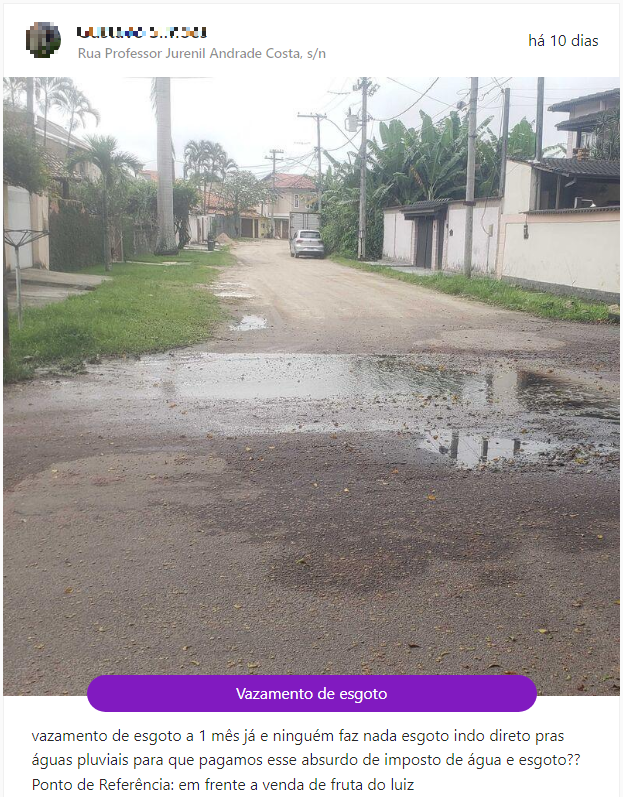
\includegraphics[width=0.7\textwidth]{images/colab_posts_taxes.png}
	\caption{Usuário do Colab denunciando problema de esgoto e fazendo referência a impostos.}
	\label{fig:colab_posts_taxes}
\end{figure}

No contexto das discussões sobre questões urbanas, observamos a presença recorrente de argumentos que abordam a questão dos altos impostos municipais e estaduais, assim como os custos associados aos serviços públicos oferecidos à população. Esses argumentos frequentemente destacam a relação intrínseca entre a carga tributária e a qualidade dos serviços públicos. Além disso, os usuários também levantam questões relacionadas à corrupção e à má gestão dos recursos públicos, que podem ser diretamente associadas à política tributária. A análise dos eventos relacionados a essa temática resumidos na \autoref{tab:eventos_populares_taxes}, revela uma tendência marcante: a maioria deles exibe scores médios negativos. Essa tendência sugere que os usuários tendem a expressar sentimentos predominantemente negativos em relação a eventos vinculados a impostos, como o IPTU e IPVA. Essa predominância de sentimentos negativos pode indicar um profundo descontentamento em relação à carga tributária vigente ou à forma como os impostos são administrados.

É importante notar que a conexão direta entre o aumento de impostos e a piora dos serviços públicos pode ser simplista. A relação entre carga tributária e qualidade dos serviços é complexa e influenciada por vários fatores, como gestão pública, alocação de recursos e eficiência administrativa. Portanto, é fundamental adotar uma abordagem mais abrangente para compreender essa interação.

\begin{figure}[htb]
	\centering
	\includegraphics[width=0.7\textwidth]{images/wordcloud_taxes.png}
	\caption{Wordcloud com palavras mais frequentes em postagens sobre Política Tributária}
	\label{fig:wordcloud_taxes}
\end{figure}

Nesse contexto, investigar as dinâmicas de pressão social relacionadas à política tributária e às questões urbanas, a fim de compreender melhor como os usuários do Colab se engajam nesse debate e como suas opiniões e sentimentos se manifestam. Ao explorar os eventos selecionados e as métricas de pressão social associadas a eles, buscamos identificar tendências, padrões e possíveis polarizações nas discussões sobre impostos e serviços públicos. Notavelmente, constatamos que, quando a persona dos usuários é identificada como \textit{complainer}, denotando uma tendência a expressar reclamações ou insatisfações individualistas, e o score de sentimento da postagem é majoritariamente negativo muitos usuários fazem referência a termos tributários, como IPTU, impostos e IPVA, em suas postagens. Essa observação sugere que, em grande parte, os usuários utilizam os impostos como justificativa para expressar seu descontentamento em relação à qualidade dos serviços públicos, argumentando que, considerando a quantidade de impostos pagos, os serviços deveriam ser de melhor qualidade. Essa análise crítica permitirá uma visão mais informada sobre as preocupações dos cidadãos em relação à política tributária e contribuirá para um diálogo mais substancial e equilibrado sobre esse tema de relevância pública.

\begin{quadro}[htb]
	\centering
	\includegraphics[width=0.7\textwidth]{images/social_barometer_taxes.png}
	\caption{Gráfico de Radar ilustrando a pressão social em relação ao tópico de Política Tributária.}
	\label{fig:social_barometer_taxes}
\end{quadro}

Para uma análise mais detalhada dos resultados do Barômetro de Pressão Social relacionados à política tributária, procedemos à categorização dos eventos em seis áreas distintas: transporte público, infraestrutura e patrimônio público, meio ambiente, saneamento básico, iluminação e energia, e saúde pública. Cada uma dessas categorias abrange eventos que foram mencionados pelos usuários e apresenta uma perspectiva única sobre como a política tributária é percebida em relação a diferentes serviços públicos e questões urbanas. As avaliações de persona e score foram realizadas para cada categoria, permitindo uma compreensão mais profunda das preocupações e sentimentos dos usuários em relação a esses tópicos específicos. A seguir, exploraremos os resultados dessas categorias e suas implicações em relação à percepção pública sobre impostos e serviços públicos.

No que diz respeito ao transporte público, os eventos relacionados a problemas como 'ônibus superlotado' 'ponto de ônibus danificado' e 'ônibus fora do horário/rota' exibem persona média próxima \textit{complainer} e scores médios negativos. Isso sugere que os usuários tendem a reclamar dessas questões, expressando sentimentos predominantemente negativos. Essas reclamações podem estar relacionadas aos altos impostos pagos pelos cidadãos. Os usuários podem argumentar que, dado o montante de impostos que pagam, esperam um serviço de transporte público de maior qualidade. Portanto, há uma correlação entre reclamações sobre transporte público e insatisfação com a política tributária, na medida em que os impostos podem ser vistos como financiadores dos serviços de transporte.

Quando examinamos eventos relacionados à infraestrutura e patrimônio público, como 'buraco nas vias' 'estação de ônibus/trem/metrô danificada' 'fiação irregular' e 'patrimônio histórico em risco' observamos uma persona média próxima \textit{complainer} e scores médios negativos. Isso indica que os usuários tendem a reclamar dessas questões e expressar sentimentos predominantemente negativos. É interessante notar que, nesse contexto, a reclamação não está diretamente relacionada aos impostos, mas sim à qualidade dos serviços públicos e à conservação da infraestrutura. No entanto, há uma conexão indireta com a política tributária, uma vez que os cidadãos podem questionar a alocação de recursos e a eficácia do gasto público, considerando os impostos que pagam.

Ao examinar eventos de Meio Ambiente, como 'Vazamento de água' e 'Mato alto', apresentam scores médios negativos, indicando uma tendência de sentimentos negativos entre os usuários. No entanto, a persona média é próxima de 1, o que sugere uma inclinação mais forte para o perfil \textit{complainer}. Nesse contexto, os usuários podem estar insatisfeitos com a gestão dos recursos públicos e, possivelmente, associando essa insatisfação aos impostos pagos.

Os dados podem ser úteis para administradores de cidades ao informar políticas públicas relacionadas ao tema. Eles devem considerar não apenas a política tributária, mas também outros fatores que afetam a prestação de serviços públicos de qualidade. Além disso, é crucial evitar generalizações simplistas que levem a discursos polarizados e à disseminação de informações imprecisas. Ao analisar criticamente as questões urbanas e a política tributária, os usuários podem contribuir de maneira mais construtiva para o debate público e para a formulação de políticas que busquem a melhoria da qualidade de vida nas cidades.

\subsection{Corrupção}
\label{sec:eventos_populares_corruption}

\begin{figure}[htb]
	\centering
	\includegraphics[width=0.7\textwidth]{images/colab_posts_corruption.png}
	\caption{Exemplo de postagem de um usuário levantando suspeitas de corrupção em um evento de zeladoria pública.}
	\label{fig:colab_posts_corruption}
\end{figure}

A corrupção é um tema recorrente nas discussões urbanas no Brasil, ligada a problemas como infraestrutura precária e serviços públicos deficientes. No Colab, observa-se uma dinâmica polarizada entre aqueles que denunciam a corrupção como causa desses problemas. A análise das métricas de pressão social disponíveis na \autoref{tab:eventos_populares_corruption} revela nuances importantes nessa dinâmica.

\begin{figure}[htb]
	\centering
	\includegraphics[width=0.7\textwidth]{images/wordcloud_corruption.png}
	\caption{Wordcloud com palavras mais frequentes em postagens sobre Corrupção}
	\label{fig:wordcloud_corruption}
\end{figure}

Usuários frequentemente mencionam palavras-chave como 'corrupção', 'propina' e 'fraude' ao discutir questões urbanas. Isso mostra que a corrupção está no centro das preocupações dos cidadãos. Eles relacionam casos de corrupção a problemas como obras de infraestrutura malfeitas e serviços públicos deficientes.

\begin{quadro}[htb]
	\centering
	\includegraphics[width=0.7\textwidth]{images/social_barometer_corruption.png}
	\caption{Gráfico de Radar ilustrando a pressão social em relação ao tópico de Corrupção.}
	\label{fig:social_barometer_corruption}
\end{quadro}

Ao analisar eventos urbanos específicos, vemos como os usuários percebem a corrupção em seu contexto. Alguns eventos têm uma persona predominantemente \textit{complainer}, como o 'Ponto de infração de trânsito recorrente', onde os usuários denunciam infrações ligadas à corrupção no sistema de fiscalização. Outros eventos, como 'Foco de mosquito da dengue/zika' e 'Comércio aberto irregularmente', também têm personas \textit{complainer}, mas com scores médios positivos, indicando que os usuários estão dispostos a oferecer soluções construtivas.

Por outro lado, eventos como 'Bloqueio na via' e 'Via de terra com desnível' têm personas \textit{complainer} com scores médios negativos, indicando alta insatisfação e falta de confiança nas autoridades em relação a essas questões. Os usuários acreditam que a corrupção contribui para a má gestão da infraestrutura.

Em resumo, a análise dos eventos relacionados à corrupção destaca a polarização desse tópico no Colab. Para os administradores das cidades, esses dados podem informar políticas públicas de diversas maneiras. Eles podem considerar a necessidade de promover transparência e responsabilidade governamental para atender às preocupações dos cidadãos. Além disso, podem buscar envolver os usuários na busca por soluções construtivas e na fiscalização das questões urbanas. Uma abordagem abrangente que leve em conta as diferentes perspectivas dos cidadãos é essencial para lidar com a corrupção e seus efeitos na vida urbana.

\subsection{Eleições e Políticos}
\label{sec:eventos_populares_polititians}

\begin{figure}[htb]
	\centering
	\includegraphics[width=0.7\textwidth]{images/colab_posts_polititians.png}
	\caption{Exemplo de postagem ironizando políticos ao fazer referência a um evento de zeladoria pública.}
	\label{fig:colab_posts_polititians}
\end{figure}

As discussões sobre eleições e políticos no contexto dos problemas urbanos no Brasil refletem uma interseção significativa entre a política e as questões que afetam diretamente a vida dos cidadãos. No Colab, um espaço digital onde os cidadãos identificam e discutem problemas nas cidades, essa conexão se torna evidente. Os usuários não apenas abordam questões relacionadas à infraestrutura e serviços públicos, mas também vinculam essas questões ao cenário político do país. Esse ambiente propicia debates intensos e frequentemente polarizados.

\begin{figure}[htb]
	\centering
	\includegraphics[width=0.7\textwidth]{images/wordcloud_polititians.png}
	\caption{Wordcloud com palavras mais frequentes em postagens sobre Eleições e Políticos}
	\label{fig:wordcloud_polititians}
\end{figure}

As métricas de pressão social da \autoref{tab:eventos_populares_polititians} demonstra alguns pontos específicos onde os usuários parecem atribuir demandas da cidade a políticos ou partidos específicos. Enquanto alguns expressam insatisfação com impostos elevados e tarifas onerosas, outros conectam os problemas urbanos às promessas e ações de políticos, destacando a ineficiência e questões políticas subjacentes. Essa polarização reflete as divisões políticas na sociedade brasileira e contribui para debates intensos sobre como a política afeta a qualidade de vida nas cidades.

Os usuários frequentemente mencionam políticos de diferentes partidos, refletindo a diversidade política da cidade. As discussões em torno de políticos e partidos podem ser calorosas e estão diretamente ligadas a questões urbanas, como infraestrutura e serviços públicos. Durante períodos eleitorais, como as eleições para prefeito e vereador, a pressão social em torno desse tópico aumenta significativamente. Os eleitores discutem candidatos, suas propostas e o histórico de mandatos anteriores. Eles também compartilham informações sobre como registrar seus votos, destacando a importância da participação cívica. A pressão social relacionada a políticos e eleições é frequentemente acompanhada de debates sobre o desempenho dos vereadores e prefeitos atuais, destacando a centralidade desses representantes municipais para os cidadãos.

\begin{quadro}[htb]
	\centering
	\includegraphics[width=0.7\textwidth]{images/social_barometer_polititians.png}
	\caption{Gráfico de Radar ilustrando a pressão social em relação ao tópico de Eleições e Políticos.}
	\label{fig:social_barometer_polititians}
\end{quadro}

A análise da pressão social relacionada ao tópico revela uma dinâmica complexa e polarizada. Alguns eventos atraem uma postura mais positiva e colaborativa (\textit{helper}), enquanto outros geram críticas intensas e insatisfação (\textit{complainer}). Esses resultados destacam que os usuários têm uma postura diversificada em relação aos problemas urbanos e que a polarização é uma característica proeminente dessas discussões.

\begin{figure}[htb]
	\centering
	\includegraphics[width=0.7\textwidth]{images/colab_posts_polititians_2.png}
	\caption{Exemplo de postagem de usuário criticando políticos.}
	\label{fig:colab_posts_polititians_2}
\end{figure}

Para administradores das cidades, esses dados podem ser valiosos para informar políticas públicas relacionadas a problemas urbanos e políticos. É importante considerar a diversidade de perspectivas e a polarização ao desenvolver estratégias para lidar com questões como infraestrutura, serviços públicos e representação política. Além disso, durante os períodos eleitorais, é fundamental promover o engajamento cívico e a transparência para fortalecer a confiança dos cidadãos nas instituições políticas. Uma abordagem equilibrada e inclusiva é essencial para encontrar soluções eficazes para os desafios urbanos.

\section{Mapeando a Opinião Pública}

O experimento de análise das discussões no Colab nos trouxe valiosos insights sobre a diversidade de perspectivas e abordagens dos usuários em relação a uma variedade de tópicos urbanos. Ao examinar os valores de persona média e score médio em eventos relacionados a pressão social, como paisagismo, meio ambiente, gentrificação, higienismo social, segurança pública, drogas, pânico moral, política tributária, corrupção e políticos, pudemos identificar tendências interessantes que lançam luz sobre a dinâmica das discussões na plataforma.

Primeiramente, ficou evidente que não existe um único tipo de evento com uma persona predominante \textit{helper} ou \textit{complainer}. A distribuição de personas e scores varia amplamente entre os eventos, refletindo a complexidade e a diversidade das questões urbanas. Isso nos leva a concluir que a comunidade do Colab aborda diferentes problemas com uma ampla gama de atitudes, desde a busca ativa por soluções até a expressão de críticas construtivas ou negativas.

Além disso, a análise revelou que mesmo nas discussões em que predominam as personas \textit{helper} ainda podem surgir críticas construtivas, e nas discussões com predominância de personas \textit{complainer} ainda podem existir elementos construtivos. Isso sugere que os usuários estão dispostos a considerar diferentes perspectivas e contribuir para melhorias, independentemente de sua atitude inicial em relação ao problema.

Quanto à polarização no Colab, observamos que, embora as discussões possam ser críticas e até mesmo negativas em alguns casos, a maioria dos usuários parece estar comprometida em abordar e resolver os desafios urbanos. A polarização pode estar presente em debates políticos e em tópicos sensíveis, como corrupção e gentrificação, mas a presença significativa de personas \textit{helper} indica uma disposição para encontrar soluções construtivas, mesmo em meio a divergências.

\begin{quadro}[htb]
	\centering
	\includegraphics[width=0.7\textwidth]{images/network_niteroi_personas_plot.png}
	\caption{Mobilidade Urbana - Helpers vs. Complainers em Niterói.}
	\label{fig:network_niteroi_personas_plot}
\end{quadro}

É interessante observar como uma abordagem de engenharia de software pode ser aplicada a um problema social complexo como a análise de pressão social hiperlocal no Colab. As heurísticas desenvolvidas no início do capítulo desempenham um papel crucial na criação de métricas quantitativas que permitem medir a opinião média e as personas dos usuários em relação a diferentes tipos de eventos de zeladoria pública. Além disso, essas heurísticas fornecem uma base sólida para a criação de representações visuais, como o gráfico de radar, que ajudam a visualizar as dinâmicas sociais de forma acessível.

A coleta de dados estruturados, através do desenvolvimento de um modelo de dados bem definido, é essencial para organizar informações relevantes, proporcionando uma compreensão clara dos elementos essenciais para a análise. Além disso, a aplicação de algoritmos de classificação e processamento de linguagem natural, como o uso de aprendizado de máquina para classificar usuários em personas e atribuir scores de sentimento às postagens, automatiza análises complexas de texto, economizando tempo e recursos.

A criação de representações visuais, como o gráfico de radar, desempenha um papel crucial na comunicação de insights complexos de maneira acessível. Essas visualizações destacam padrões e tendências, facilitando a tomada de decisões informadas. A abordagem de engenharia de software também permite a iteração e o aprendizado contínuo, possibilitando melhorias constantes no sistema com base em resultados e em evoluções nas dinâmicas sociais.

A integração eficaz das análises e insights com os tomadores de decisão, como agências governamentais e organizações da sociedade civil, é fundamental para garantir que os resultados sejam aplicados para informar políticas e ações práticas. Essa abordagem colaborativa promove uma governança mais informada e eficaz, aproveitando a tecnologia para compreender e resolver problemas sociais complexos.

A aplicação de abordagens de engenharia de software à análise de problemas sociais complexos é uma maneira eficaz de aproveitar a tecnologia para compreender melhor as dinâmicas sociais, identificar áreas de preocupação e promover o envolvimento cidadão. Além disso, a abordagem iterativa permite que o sistema evolua e se adapte às necessidades em constante mudança das comunidades urbanas, contribuindo para uma governança mais informada e eficaz.

O experimento nos ensinou que a plataforma Colab é um reflexo da complexidade das questões urbanas e das opiniões diversificadas de seus usuários. Podemos aprender que a diversidade de perspectivas é uma força, pois permite a consideração de uma ampla gama de soluções para os problemas urbanos. A análise também nos lembra da importância de um diálogo construtivo e da busca de soluções colaborativas para promover uma cidade mais eficiente, segura e inclusiva.

Em um mundo onde as divisões são cada vez mais comuns, o Colab nos mostra que, apesar das diferenças, as comunidades podem se unir em busca de um objetivo comum: tornar as cidades melhores lugares para se viver. Portanto, ao continuar a incentivar o diálogo e a colaboração, o Colab pode desempenhar um papel importante na melhoria das condições urbanas e na promoção do bem-estar de todos os cidadãos.

\section{Aspectos hiperlocais}

Ao explorarmos a dinâmica da pressão social e sua manifestação por meio de discussões e relatos de problemas urbanos no Colab, entendemos como os usuários da plataforma expressam preocupações, sentimentos e opiniões sobre uma variedade de tópicos, destacando as questões mais relevantes e polarizadoras que afetam suas comunidades. Agora, avançaremos na análise para ressaltar o aspecto hiperlocal, concentrando-nos na comparação entre as três cidades analisadas.

Considerar aspectos hiperlocais, é reconhecer que diferentes localidades podem reagir de maneiras diversas aos mesmos problemas urbanos. Niterói e Mesquita, situadas no estado do Rio de Janeiro, e Santo André, localizada em São Paulo, compartilham desafios comuns enfrentados por muitas cidades brasileiras, como infraestrutura, segurança pública e qualidade de vida. No entanto, a percepção e a priorização desses desafios podem variar significativamente entre essas duas cidades. Da mesma forma, diferentes bairros da mesma cidade podem ter preocupações e necessidades distintas criando um padrão de criação de demandas diferente entre as regiões. É importante notar também que a percepção de certos tipos de problemas pode ser palpável para alguns grupos sociais e invisível para outros. O importante é que o aplicativo Colab mantém todas essas demandas criadas através de eventos de zeladoria geo-referenciadas, o que permite uma análise hiperlocal.

Para entender melhor essas nuances, analisamos os tipos de eventos mais criados em Niterói, Mesquita e Santo André. Embora ambos os municípios enfrentem problemas relacionados a buracos nas vias e lâmpadas apagadas à noite, a classificação dos tipos de eventos revela diferenças marcantes. Niterói apresenta uma alta incidência de eventos relacionados a problemas nas vias, como 'Buraco nas vias' 'Calçada irregular' e 'Ponto de infração de trânsito recorrente'. Esses eventos estão diretamente ligados à mobilidade urbana e à infraestrutura viária, indicando uma preocupação significativa dos cidadãos em relação a essa questão. Portanto, um tópico de pressão social relevante para Niterói é a 'Mobilidade Urbana'. Mesquita tem um grande número de eventos relacionados à natureza e ao meio ambiente, como 'Poda de árvore' e 'Mato alto'. Esses eventos indicam uma preocupação com a preservação ambiental e o paisagismo urbano. Portanto, um tópico de pressão social relevante para Santo André é o 'Meio Ambiente'. Santo André enfrenta desafios relacionados à limpeza e à infraestrutura urbana, como 'Entulho na calçada/via pública' e 'Esgoto a céu aberto'. Esses problemas podem afetar diretamente a saúde pública dos cidadãos. Portanto, um tópico de pressão social relevante para Santo André é a 'Saúde Pública'.

Embora esses tópicos sejam relevantes para as três cidades, a análise revela que cada uma delas tem uma percepção e uma priorização únicas dos problemas urbanos. Essas diferenças podem ser atribuídas a uma variedade de fatores, como a infraestrutura urbana, a composição demográfica e a cultura local. A análise também destaca a importância de uma abordagem hiperlocal para entender melhor as necessidades e os desafios de cada comunidade. Ao considerar essas nuances, os gestores públicos podem tomar decisões mais informadas e eficazes, contribuindo para uma governança mais inclusiva e participativa. Essa análise inicial destaca como as diferentes cidades reagem e percebem os problemas urbanos de maneira única, mesmo quando enfrentam desafios semelhantes. A partir desses dados, podemos aprofundar nossa investigação para entender melhor os fatores locais que moldam essas percepções e prioridades, contribuindo para uma compreensão mais abrangente da pressão social hiperlocal e suas implicações na gestão urbana.

A partir da definição dos tópicos a serem analisados, desenvolvemos uma metodologia para criar visualizações de pressão social hiperlocal utilizando dados de geolocalização de eventos postados em mídias sociais. A metodologia emprega bibliotecas como Folium e Bokeh para a geração dos mapas interativos e gráficos de rede. Primeiramente, os dados são filtrados para uma região de interesse, no caso, a cidade de Santo André. Em seguida, são selecionadas palavras-chave relevantes relacionadas à saúde pública, tais como 'hospital' 'pronto socorro' 'vacinação' entre outras. Eventos que não estão diretamente relacionados a essas palavras-chave são excluídos do conjunto de dados. A visualização inclui dois componentes principais: mapas de calor (heatmaps) e um gráfico de rede (network).

Para os heatmaps, a ponderação é ajustada com base em uma métrica de sentimento, e um mapa base é criado, centrado na média das coordenadas geográficas dos eventos selecionados. Os dados ponderados são utilizados para gerar o mapa de calor, com uma escala de cores que indica o sentimento dos eventos.

No gráfico de rede, as conexões entre os eventos e os usuários que os postaram são identificadas e representadas. A biblioteca NetworkX é utilizada para criar o gráfico, e os nós são posicionados com base nas coordenadas geográficas dos eventos. Uma adição importante à visualização é a coloração dos nós com base nas personas identificadas: azul para os \textit{helpers}  e vermelho para os \textit{complainers}. Além disso, o polígono da cidade é utilizado como referência para centralizar tanto o mapa de rede quanto os pontos de eventos. Isso contribui significativamente para destacar a localização dos eventos em relação à área geográfica da cidade, possibilitando uma análise mais detalhada das dinâmicas de saúde pública em nível hiperlocal.

Essas visualizações permitem a identificação de padrões de atividade relacionados aos tópicos de pressão social a nível hiperlocal. Os heatmaps revelam áreas de maior atividade e sentimentos associados aos eventos, permitindo uma compreensão mais granularizada das preocupações da comunidade em áreas específicas da cidade. O gráfico de rede, por sua vez, mostra como os eventos e usuários estão interconectados, possibilitando a identificação de influenciadores ou grupos de interesse em questões de saúde pública. A combinação de heatmaps e gráficos de rede fornece insights valiosos para formuladores de políticas públicas, pesquisadores e profissionais de saúde na tomada de decisões e no planejamento de intervenções em saúde pública a nível hiperlocal.

\subsection{Mobilidade Urbana em Niterói}

A análise dos dados de pressão social sobre mobilidade urbana em Niterói da \autoref{tab:eventos_populares_mobility_niteroi} revela as percepções dos cidadãos em relação a esse tema. Podemos notar uma divisão entre "complainers" e "helpers" em relação a diferentes eventos, refletindo as atitudes da comunidade.

\begin{quadro}[htb]
	\centering
	\includegraphics[width=0.7\textwidth]{images/heatmap_niteroi.PNG}
	\caption{Heatmap de Pressão Social para Mobilidade Urbana em Niterói}
	\label{fig:heatmap_niteroi}
\end{quadro}

\begin{figure}[htb]
	\centering
	\includegraphics[width=0.7\textwidth]{images/wordcloud_niteroi.png}
	\caption{Palavras mais frequentes nas postagens de Niterói}
	\label{fig:wordcloud_niteroi}
\end{figure}

Eventos com uma persona predominantemente \textit{complainer} indicam insatisfações, como o caso do evento relacionado à condição sanitária irregular de estabelecimentos na cidade. Por outro lado, eventos com uma persona predominantemente \textit{helper}, como aqueles relacionados a infrações de trânsito, demonstram a disposição da comunidade em colaborar para melhorar a situação.

\begin{quadro}[htb]
	\centering
	\includegraphics[width=0.7\textwidth]{images/social_barometer_niteroi.png}
	\caption{social barometer niteroi}
	\label{fig:social_barometer_niteroi}
\end{quadro}

Os eventos mais populares, como buracos nas vias, refletem a importância da infraestrutura viária e segurança no trânsito para os cidadãos de Niterói. A presença de eventos relacionados à acessibilidade também destaca desafios significativos nessa área, chamando a atenção para a necessidade de políticas que melhorem a acessibilidade urbana.

Além disso, os dados revelam sentimentos positivos e negativos relacionados a diferentes eventos, com a comunidade expressando insatisfação em relação à poluição sonora e falta de energia, enquanto demonstra apoio a iniciativas de arborização.

Para os administradores da cidade, esses insights podem informar políticas públicas eficazes. Eles podem priorizar a regulamentação de estabelecimentos com condições sanitárias precárias, promover campanhas de conscientização sobre as leis de trânsito e investir na manutenção viária. Além disso, medidas para melhorar a acessibilidade e reduzir a poluição sonora podem ser implementadas com base nos dados coletados.

Em resumo, essas métricas de pressão social podem orientar as autoridades locais na criação de políticas públicas que promovam uma mobilidade urbana mais segura, acessível e eficiente em Niterói, atendendo às necessidades e preocupações da comunidade.

\subsection{Meio Ambiente em Mesquita}
A análise dos dados sobre o meio ambiente em Mesquita revela informações cruciais sobre as preocupações e percepções da comunidade local. Conforme apresentado na \autoref{tab:eventos_populares_mesquita}, diferentes eventos, como descarte irregular de lixo, poluição do ar e desmatamento, foram analisados para identificar tendências e opiniões da comunidade. Alguns eventos são relatados de maneira crítica e negativa, enquanto outros são vistos de forma mais positiva.

\begin{quadro}[htb]
	\centering
	\includegraphics[width=0.7\textwidth]{images/heatmap_mesquita.PNG}
	\caption{Heatmap de Pressão Social para Meio Ambiente em Mesquita}
	\label{fig:heatmap_mesquita}
\end{quadro}

Eventos como 'Descarte irregular de lixo' e 'Ponto de queimada irregular recorrente' têm uma perspectiva predominantemente negativa e pontuações negativas. Por outro lado, eventos como 'Limpeza de Canais' e 'Poda de árvore' são relatados de maneira mais positiva, com pontuações positivas. A análise dos eventos mais frequentes mostra que 'Descarte irregular de lixo' e 'Ponto de queimada irregular recorrente' são as principais fontes de insatisfação na comunidade.

\begin{quadro}[htb]
	\centering
	\includegraphics[width=0.7\textwidth]{images/social_barometer_mesquita.png}
	\caption{social barometer mesquita}
	\label{fig:social_barometer_mesquita}
\end{quadro}

\begin{figure}[htb]
	\centering
	\includegraphics[width=0.7\textwidth]{images/wordcloud_mesquita.png}
	\caption{Wordcloud com palavras mais frequentes nas postagens de Mesquita}
	\label{fig:wordcloud_mesquita}
\end{figure}

Esses dados podem ser usados pelos administradores da cidade para informar políticas públicas relacionadas ao meio ambiente. Eles destacam a necessidade de abordar o descarte inadequado de resíduos sólidos e a ocorrência de queimadas irregulares como prioridades. Além disso, a comunidade demonstra apoio a ações como a poda de árvores e a conservação da via pública, indicando áreas onde investimentos e esforços positivos podem ser direcionados para melhorar a qualidade de vida e a sustentabilidade ambiental na região. A diversidade de perspectivas ressalta a importância de envolver ativamente a comunidade na proteção e preservação ambiental.

\subsection{Saúde Pública em Santo André}

A análise da pressão social relacionada à saúde pública em Santo André conforme a \autoref{tab:eventos_populares_sa} resume alguma das preocupações específicas dos usuários sobre esse tema. Os eventos relatados, desde infraestrutura inadequada até problemas de higiene e segurança, refletem a complexidade dessas preocupações.

\begin{quadro}[htb]
	\centering
	\includegraphics[width=0.7\textwidth]{images/heatmap_santo_andre.PNG}
	\caption{Heatmap de Pressão Social para Saúde Pública em Santo André}
	\label{fig:heatmap_santo_andre}
\end{quadro}

Alguns eventos, como 'Coleta de container' e 'Limpeza de área pública', estão associados a preocupações legítimas da comunidade em relação à falta de serviços e manutenção adequados na cidade. Por outro lado, eventos como 'Falta de água' são percebidos como situações que requerem intervenção positiva para resolver o problema. No entanto, também existem eventos com críticas significativas em relação à infraestrutura de saúde e à conformidade com regulamentos, indicando uma insatisfação com essas áreas.

\begin{quadro}[htb]
	\centering
	\includegraphics[width=0.7\textwidth]{images/social_barometer_santo_andre.png}
	\caption{social barometer santo andré}
	\label{fig:social_barometer_santo_andre}
\end{quadro}

No contexto da pandemia de COVID-19, os eventos mais populares, como 'Lixo' e 'Aglomeração de pessoas', ganham ainda mais relevância e urgência. 'Aglomeração de pessoas' reflete a disposição da comunidade para colaborar, mas ainda há preocupações substanciais em relação à aglomeração. 'Lixo' apresenta uma mistura de percepções positivas e críticas, indicando a necessidade de melhorias na gestão de resíduos.

\begin{quadro}[htb]
	\centering
	\includegraphics[width=0.7\textwidth]{images/network_santo_andre_personas_map.png}
	\caption{Rede de eventos populares relacionados a Saúde Pública em Santo André}
	\label{fig:network_santo_andre_personas_map}
\end{quadro}

\begin{figure}[htb]
	\centering
	\includegraphics[width=0.7\textwidth]{images/wordcloud_santo_andre.png}
	\caption{Palavras mais frequentes nas postagens de Santo André}
	\label{fig:wordcloud_santo_andre}
\end{figure}

Em resumo, os dados refletem a complexidade da saúde pública em Santo André, com a comunidade demonstrando uma consciência aguçada das questões que afetam seu bem-estar. As reclamações estão concentradas em áreas críticas, e o diálogo positivo em alguns eventos indica um desejo de cooperação para resolver esses problemas. Para os administradores das cidades, esses dados podem ser usados para informar políticas públicas relacionadas à saúde pública, identificando áreas de foco e necessidades específicas da comunidade.

\section{Trabalhos Futuros}

Em um contexto acadêmico, a abordagem central deste estudo reside na análise das câmaras de eco e na concepção do Colab como um barômetro social hiperlocal. Essa perspectiva oferece uma visão singular e abrangente das interações e percepções das comunidades locais em relação a tópicos polarizadores. No entanto, vale ressaltar que essa metodologia não se limita a seu emprego na pesquisa de câmaras de eco, sendo passível de extensão para diversas outras áreas de estudo.

A observação do Colab como um barômetro social hiperlocal implica em uma compreensão detalhada das opiniões, discussões e manifestações das comunidades locais em relação a questões específicas. Nesse contexto, a polarização emerge como um tema fundamental, visto que a plataforma proporciona uma visão inédita das dinâmicas de polarização no nível mais próximo da comunidade, indo além das análises tradicionais de polarização em escala mais ampla.

Essa abordagem também sugere que a pressão social hiperlocal proproem uma dimensão rica e relevante que pode ser investigada em outros contextos de pesquisa. Embora este estudo se concentre nas câmaras de eco e nas dinâmicas sociais específicas do Colab, é possível extrapolar essas heurísticas e metodologias para áreas de estudo diversas. Assim, abre-se a perspectiva para futuros trabalhos que explorem como a pressão social hiperlocal pode ser aplicada e analisada em campos como políticas públicas, meio ambiente, saúde pública, desenvolvimento urbano, engajamento cívico e conflitos sociais, entre outros.

Em pesquisas futuras, há um vasto campo a ser explorado no aprimoramento das heurísticas e métodos de análise da pressão social hiperlocal, especialmente no contexto de plataformas como o Colab. Uma das direções promissoras seria a incorporação de dimensões temporais e geolocalização de maneira mais robusta. Isso poderia ser alcançado através do desenvolvimento de algoritmos de análise de séries temporais para monitorar a evolução das discussões e do sentimento em torno de tópicos específicos ao longo do tempo. Compreender como as percepções e prioridades mudam sazonalmente ou em resposta a eventos específicos seria fundamental para uma análise mais holística. Além disso, a geolocalização desempenha um papel crítico na pressão social hiperlocal. A capacidade de mapear a localização precisa de eventos e discussões poderia permitir uma análise mais granular das dinâmicas das comunidades urbanas. Seria interessante explorar técnicas avançadas de geolocalização, como a análise de dados geoespaciais, para identificar padrões de pressão social em áreas urbanas específicas. Isso poderia ajudar as autoridades locais a direcionar recursos de forma mais eficaz e tomar decisões informadas sobre políticas públicas.

Também, vale a pena considerar a extensibilidade dessas heurísticas para outras redes sociais e plataformas além do Colab. A pressão social hiperlocal não é exclusiva de uma única plataforma, e compreender como ela se manifesta em diferentes contextos online poderia fornecer insights valiosos sobre o comportamento cívico e a participação pública em ambientes digitais variados. Isso abriria a porta para a criação de um framework mais amplo e aplicável a diversas situações. Outra área de pesquisa interessante seria a avaliação das implicações políticas e de governança da pressão social hiperlocal. Como as percepções locais podem influenciar as decisões políticas e a prestação de serviços públicos? Investigar como as vozes hiperlocais impactam as políticas urbanas e como as autoridades respondem a essas pressões seria um campo de estudo crítico para aprimorar a governança democrática.

A compreensão das dinâmicas da pressão social hiperlocal pode ser aplicada para informar a tomada de decisões políticas e a prestação de serviços públicos em nível local. Os governos municipais podem usar essa análise para identificar as principais preocupações dos cidadãos e a eficácia de suas políticas, adaptando-as de acordo com as demandas locais. Em estudos relacionados ao meio ambiente e desastres naturais, a pressão social hiperlocal pode ser usada para rastrear as preocupações e percepções das comunidades locais. Isso permite uma resposta mais eficaz a eventos climáticos extremos, poluição e outras questões ambientais. A análise da pressão social hiperlocal pode ser aplicada ao monitoramento de questões de saúde pública, como surtos de doenças infecciosas. A detecção rápida de preocupações da comunidade em relação à saúde pode ajudar as autoridades de saúde a tomar medidas preventivas e educativas. No contexto do desenvolvimento urbano, a pressão social hiperlocal pode ser usada para avaliar o impacto de projetos de infraestrutura, como construção de estradas, expansão de transporte público e desenvolvimento imobiliário. Isso permite uma análise mais detalhada das preocupações e necessidades das comunidades afetadas. Em estudos sobre conflitos e tensões sociais, a pressão social hiperlocal pode ser usada para identificar pontos de atrito em comunidades específicas. Isso pode ajudar na prevenção de conflitos e na promoção da coesão social.

Por fim, considerando a crescente importância da inteligência artificial e da análise de big data, explorar como essas tecnologias podem ser aplicadas de forma ética e eficaz na detecção e análise da pressão social hiperlocal é uma área promissora de pesquisa. O desenvolvimento de ferramentas automatizadas para identificar tópicos de pressão e monitorar o sentimento em tempo real poderia revolucionar a forma como as cidades respondem às demandas de seus cidadãos. Há uma série de oportunidades empolgantes para aprimorar nossas abordagens de análise da pressão social hiperlocal, incorporando dimensões temporais, geolocalização e estendendo essas heurísticas para diferentes plataformas e contextos. Isso não apenas enriqueceria nosso entendimento das comunidades urbanas, mas também teria implicações práticas significativas para a governança local e o envolvimento cívico.

\section{Conclusões}

No decorrer deste capítulo, exploramos as dinâmicas da opinião pública no Colab, uma plataforma que abriga discussões sobre tópicos urbanos diversos. Nossas análises revelaram uma diversidade de perspectivas e abordagens por parte dos usuários em relação a questões urbanas. Observamos que não há uma única persona predominante, variando amplamente entre eventos, refletindo a complexidade das questões urbanas. Isso indica que a comunidade do Colab lida com diferentes problemas de maneiras variadas, desde a busca por soluções até a expressão de críticas construtivas ou negativas.

Surpreendentemente, mesmo nas discussões em que predominam personas \textit{helper}, ainda podem surgir críticas construtivas, e vice-versa. Isso demonstra a disposição dos usuários em considerar diferentes perspectivas e contribuir para melhorias, independentemente de sua atitude inicial em relação ao problema. Além disso, apesar de algumas polarizações em debates políticos e tópicos sensíveis, a maioria dos usuários parece comprometida em abordar e resolver os desafios urbanos. A presença de personas \textit{helper} indica uma disposição para encontrar soluções construtivas, mesmo em meio a divergências.

A aplicação de abordagens de engenharia de software foi essencial para nossa análise, permitindo-nos desenvolver heurísticas para medir a opinião média e as personas dos usuários em relação a diferentes eventos urbanos. Essas heurísticas serviram de base para representações visuais, como o gráfico de radar, que auxiliaram na visualização das dinâmicas sociais de forma acessível. Além disso, a coleta de dados estruturados por meio de um modelo bem definido foi fundamental para organizar as informações e facilitar a análise. Integrando a tecnologia de aprendizado de máquina na forma de algoritmos de classificação e processamento de linguagem natural, automatizamos a análise de texto, economizando tempo e recursos. Isso nos permitiu examinar um grande volume de dados em larga escala.

Aqui reside uma conexão profunda entre a fenomenologia e a engenharia de software. Assim como a fenomenologia busca compreender as experiências subjetivas de indivíduos, nossa abordagem de engenharia de software nos permitiu mergulhar profundamente nas experiências dos usuários do Colab, revelando as nuances de suas interações e perspectivas. Ao aplicar heurísticas para medir opiniões e personas, criamos uma lente através da qual podemos observar as complexidades das redes sociais em escala.

Além disso, reconhecemos a importância de integrar os resultados de nossa análise com os tomadores de decisão, como agências governamentais e organizações da sociedade civil. Isso garante que nossas descobertas sejam utilizadas para informar políticas e ações práticas, promovendo uma governança mais informada e eficaz.

A análise também nos levou a explorar o fenômeno da polarização, que é amplamente observado em ambientes digitais, como redes sociais. Identificamos como as plataformas digitais podem contribuir para a formação de câmaras de eco e bolhas de filtro, reforçando crenças preexistentes e restringindo a exposição a diferentes perspectivas. No entanto, também reconhecemos que o ciberespaço, como definido por Levy, é um ambiente multifacetado, onde diversas vozes e visões coexistem.

Levy nos lembra que a cibercultura é caracterizada pela diversidade de atores, projetos e interpretações, frequentemente em oposição. O ciberespaço, apesar de desafios, oferece oportunidades para o diálogo e a colaboração entre diferentes perspectivas culturais. Isso é particularmente relevante no contexto do Colab, onde a diversidade de perspectivas é uma força que permite a consideração de uma ampla gama de soluções para os problemas urbanos.

Ao incorporar a análise de sentimentos e personas dos usuários em nossa compreensão do Colab, estamos agregando uma dimensão adicional à nossa capacidade de medir a pressão social hiperlocal. Isso nos permite identificar áreas de polarização e tensão dentro da comunidade, bem como oportunidades para promover o diálogo e a colaboração. A abordagem de Levy à cibercultura destaca a interconexão e a valorização da diversidade de perspectivas, e o Colab tem o potencial de se tornar um espaço inclusivo para o diálogo cidadão e a construção de comunidades informadas e coesas.

Em última análise, o Colab, como um 'barômetro social hiperlocal' e uma plataforma de cidadania, tem o potencial de desempenhar um papel crucial na promoção da participação cidadã, no engajamento construtivo e na melhoria das condições urbanas. À medida que continuamos a valorizar a diversidade de perspectivas e a buscar soluções colaborativas, podemos avançar na construção de cidades mais eficientes, seguras e inclusivas, em um ciberespaço que amplifica tanto os desafios quanto as oportunidades da opinião pública. Este capítulo nos conduziu à compreensão de que o Colab é um espaço de convergência, onde perspectivas culturais variadas têm a oportunidade de dialogar e colaborar. A diversidade de vozes é a essência da cibercultura, e o Colab é um exemplo poderoso disso.

No próximo capítulo, continuaremos a explorar a complexidade das redes sociais, mas com um foco específico na detecção de câmaras de eco. Essa pesquisa se conecta diretamente ao nosso experimento atual, onde desenvolvemos heurísticas para medir a opinião média e as personas dos usuários em relação a diferentes tipos de eventos. As heurísticas e os insights obtidos até agora servirão como base fundamental para a próxima etapa de nossa investigação.

Além disso, nosso conjunto de dados abrange não apenas os eventos criados pelos usuários, classificados por score e persona, mas também inclui informações detalhadas sobre os relacionamentos de rede social entre os usuários das três cidades, revelando os usuários mais influentes, cada seguidor e quantos usuários cada pessoa segue além dos tipos de eventos com os quais interagem. Cada evento também é enriquecido com comentários e likes, proporcionando uma visão mais completa das interações dos usuários. Com base nesses dados e nas heurísticas criadas a partir deles, seremos capazes de inferir não apenas a opinião média dos usuários em relação a diversos tipos de evento, mas também avaliar a homogeneidade de opiniões com base no tipo de evento com o qual cada usuário interage com mais frequência e compará-lo com o tipo de evento mais interagido pelos membros de sua rede social. Com cada evento, comentário ou interação, os usuários não apenas expressam uma opinião, mas também se engajam em um processo de co-criação e interpretação de significado no ciberespaço. Portanto, as ideias de barômetro social hiperlocal, pressão social e detecção de câmaras de eco estão intrinsecamente conectadas porque elas refletem as dinâmicas e nuances das relações humanas que se desdobram no ciberespaço. O conceito de 'barômetro social hiperlocal' captura a essência de como as interações individuais se somam para criar um panorama mais amplo da opinião pública em uma região específica. Ao mesmo tempo, a pressão social revela como os usuários influentes podem moldar ou direcionar as opiniões e interações dentro de suas redes. Finalmente, a detecção de câmaras de eco é uma consequência direta dessas interações, mostrando como grupos de usuários podem se tornar insulares em suas opiniões, reforçando crenças e perspectivas semelhantes.

Dentro dessa complexa teia de relacionamentos e interações, um usuário não é apenas um ponto de dados, mas uma entidade viva que busca conexão, expressão e entendimento. Os dados que coletamos e as heurísticas que aplicamos, portanto, não são meros exercícios técnicos, contudo, é fundamental lembrar que por trás desses dados, existem indivíduos com experiências reais e tangíveis. O pensamento de Heidegger sobre a 'técnificação das mãos' sugere uma preocupação com a maneira pela qual a tecnologia pode distanciar o ser humano de uma vivência autêntica do mundo. Quando um usuário do Colab cria um evento ou interage na plataforma, essa 'técnificação' pode estar presente, influenciando como ele percebe e se relaciona com o espaço digital. Nesse sentido, a própria criação de heurísticas e o uso da engenharia de software podem ser vistos como uma extensão desse processo de 'técnificação'. Por outro lado, Merleau-Ponty, com sua ênfase na corporeidade e percepção, serve como um lembrete de que as interações no Colab são manifestações de experiências corpóreas e perceptivas dos usuários.

A polarização, as câmaras de eco e até mesmo as análises de sentimentos não são meros produtos técnicos, mas emergem das experiências vividas e sentidas das pessoas. Ao avançarmos na integração entre engenharia de software e fenomenologia, é crucial lembrar que cada clique, postagem ou interação no Colab tem sua origem na experiência humana. Deste modo, nossas análises, embora apoiadas por ferramentas tecnológicas sofisticadas, devem sempre manter a centralidade do ser humano e suas experiências. Assim, mesmo quando exploramos as complexidades técnicas e analíticas, reconhecemos que elas servem para nos aproximar, e não distanciar, das nuances e riquezas da experiência humana no ciberespaço e na vida real.